\section{Methods}
\label{hptpcPaper:sec:Methods}

    \subsection{CERN Beam Test}
    The beam test took place in the 0.8~GeV T10 beam line, East Area at the Proton Synchrotron in CERN from the 15th August to the 18th September 2018.
    The primary experimental setup for the data taking period is shown in figure~\ref{fig:setup}.
    \begin{figure}
    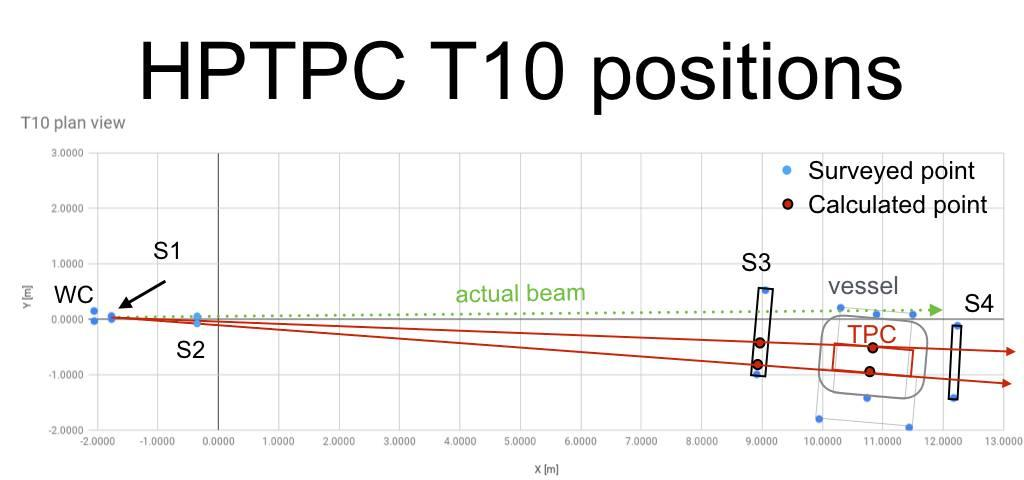
\includegraphics[width=1.0\linewidth]{files/Figures/T10Diagram.jpg}
    	\caption{Beam test configuration}
    		\label{fig:setup}
    \end{figure}
    The centre of the HPTPC Prototype was placed 13~m from the wire chamber at the beam entrance. 
    3 Time of Flight constituents, labeled S1 to S3, were placed upstream of the TPC, while the 4th, labeled S4, was placed directly downstream.
    Both the TPC and Time of Flight systems were placed at an off axis angle with respect to the direction shown by the green arrow.
    Additionally, a variable number of blocks of acrylic moderator, shown in Figure~\ref{fig:modblocks}, were placed in the beamline, upstream of S1.
      \begin{figure}
      \centering
    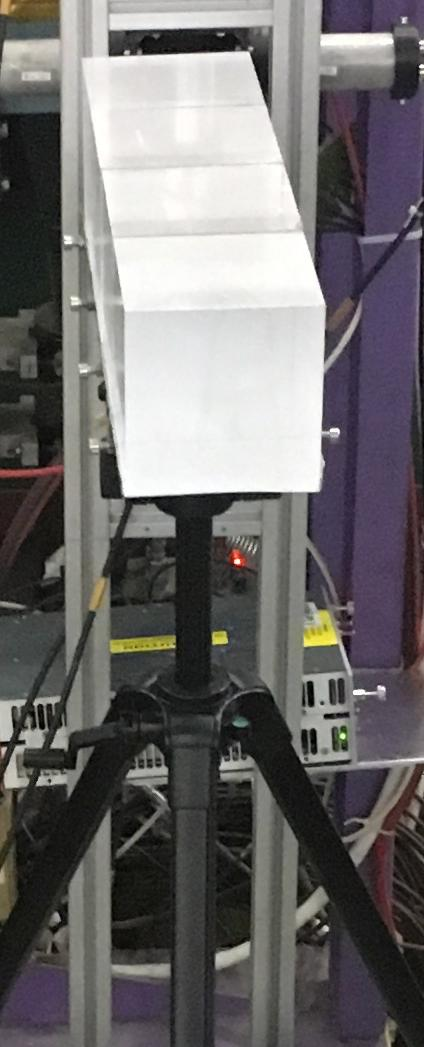
\includegraphics[width=0.2\linewidth]{files/Figures/ModeratorBlocks.jpg}
    	\caption{Acrylic Moderator Blocks}
    		\label{fig:modblocks}
    \end{figure}
    
    Moderator blocks were used in order to cause a spread in the incoming beam.
    The blocks cause protons to scatter through a larger angle than pions and other MIPs, increasing the off-axis proton pion ratio.
    The effect of this, together with placing the TPC and ToF systems off axis was to allow a measurement of protons with a lower pion background.
    This technique also had the effect of reducing the average momentum of the measured particles.
    Data were taken for 0, 1, 2, 3, and 4 moderator blocks in turn.
    The beam ran with an energy of 0.8~GeV, and primarily comprised protons and pions, as well as muons and electrons. 
    Beam spills were approximately 500~ms in length, with 5-10~s between spills.
    The ratio of protons to pions expected in the T10 beam  is shown in figure~\ref{beamcharacteristics}.
      \begin{figure}
      \centering
    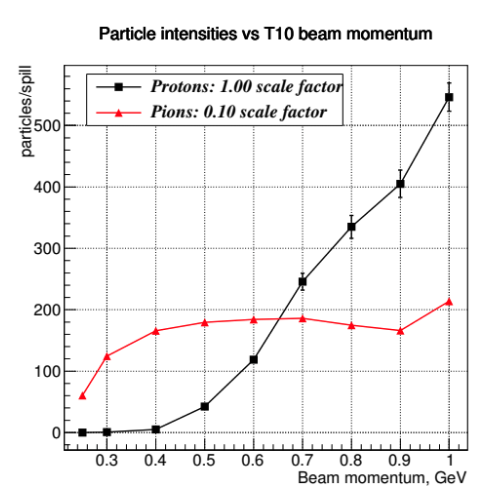
\includegraphics[width=0.6\linewidth]{files/Figures/offaxismeasurement.png}
    	\caption{T10 beam constituents (REFERENCE NEEDED)}
    		\label{fig:beamcharacteristics}
    \end{figure}
    
    
	\subsection{Upstream Time of Flight instrumentation (S1-3)}
    The upstream time of flight system was composed of the following constituents:
    S1 and S2, a 4~cm by 4~cm plastic counter with 30~ps resolution and a trigger counter resepctively.
    S1 and S2 are shown in figure~\ref{}.
    These were placed within 2~m of the beam entrance
    S3, a SHiP prototype wall produced by the Université de Genève. 
    The wall was 168~cm by 110~cm made up of 20 plastic scintillator bars with 90~ps timing resolution.
    The S3 wall was placed directly upstream of the TPC.
    S3 is shown in figure~\ref{}.

	\subsection{Downstream Time of Flight instrumentation (S4)}
	
    The downstream time of flight system, $S4$, consists of 10 bars of Nuvia plastic scintillator, which form the detector medium. 
    Attached to either end of each of these scintillator bars is a 5" Hamamatsu R6594 photomultiplier tube. 
    The bars are arranged in two rows of five, such that there is complete coverage for any beam particles incident upon the detector. 
    Diagrams of the $S4$ wall, along with its dimensions are presented in figure~\ref{fig:dstofFront} and~\ref{fig:dstofDiagonal}.
    The time resolution of the bars and PMTs was measured to be 1~ns. The corresponding spatial resolution of the bars and PMTs was measured to be 8.3~cm.
    
    \begin{figure}[ht]    
    	\begin{minipage}[t]{.48\textwidth}
    		\centering
    		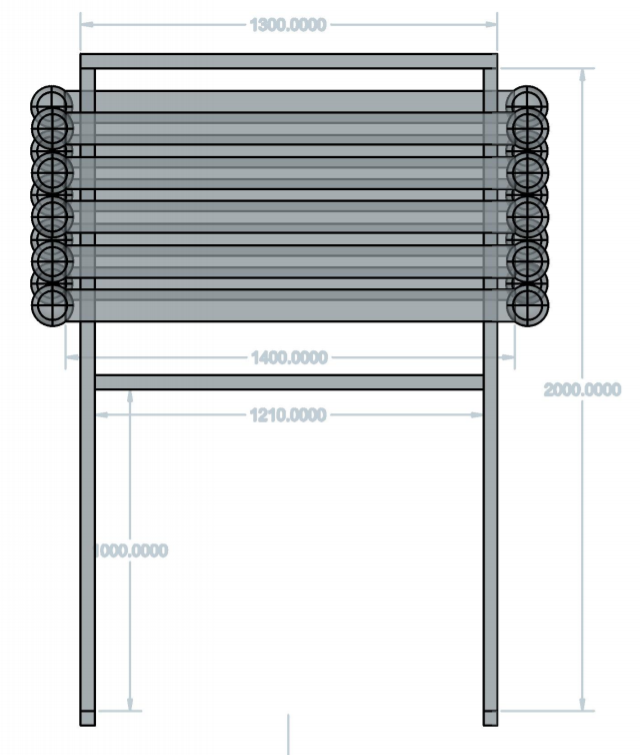
\includegraphics[width=0.6\linewidth]{files/Figures/dstofFront.png}
    		\caption{Front view of the downstream time of flight system}
    		\label{fig:dstofFront}
    	\end{minipage}
    	\hspace{0.3cm}
    	\begin{minipage}[t]{.48\textwidth}
    		\centering
    		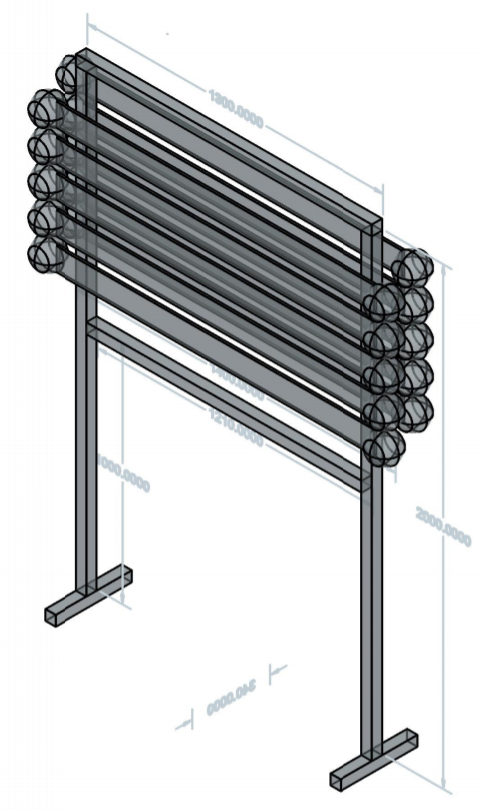
\includegraphics[width=0.45\linewidth]{files/Figures/dstofDiag.png}
    		\caption{Diagonal view of the downstream time of flight system showing more clearly the two rows of scintillator bars and photomultiplier tubes}
    		\label{fig:dstofDiagonal}
    	\end{minipage}
    \end{figure}
    
    All 20 of the photomultiplier tubes have their anode signals read out using NIM discriminators which are then fed into a time-to-digital converter. 
    A signal (i.e. an incident particle of any kind) in $S4$ was considered to have occurred if a signal was seen in both photomultiplier tubes on the same bar within 20~ns of each other.
    
    Additionally, a signal was also fed into the same time-to-digital converter whenever there was a coincidence between the $S1$ and $S2$ timing points. 
    When calculating the time of flight of a given particle, this time of coincidence was used as first timing point.
    
    \subsection{The HPTPC Prototype}
    The prototype was built at Royal Holloway, University London.
    The steel vessel was rated to 6~barA of pressure, and the walls of the vessel were 4~cm thick (THIS NEEDS CHECKING).
    The TPC comprised thin steel mesh electrodes (one cathode and three anodes), and 12 copper rings to create the uniform drift field.
    The drift distance produced was 48~cm, with the anodes separated by 1~mm.
    Data taking with the TPC made use of both optical and charge readout.
    The vessel, electrodes, and drift region of the TPC are shown in figure~\ref{fig:TPC}
    
     \begin{figure}
      \centering
    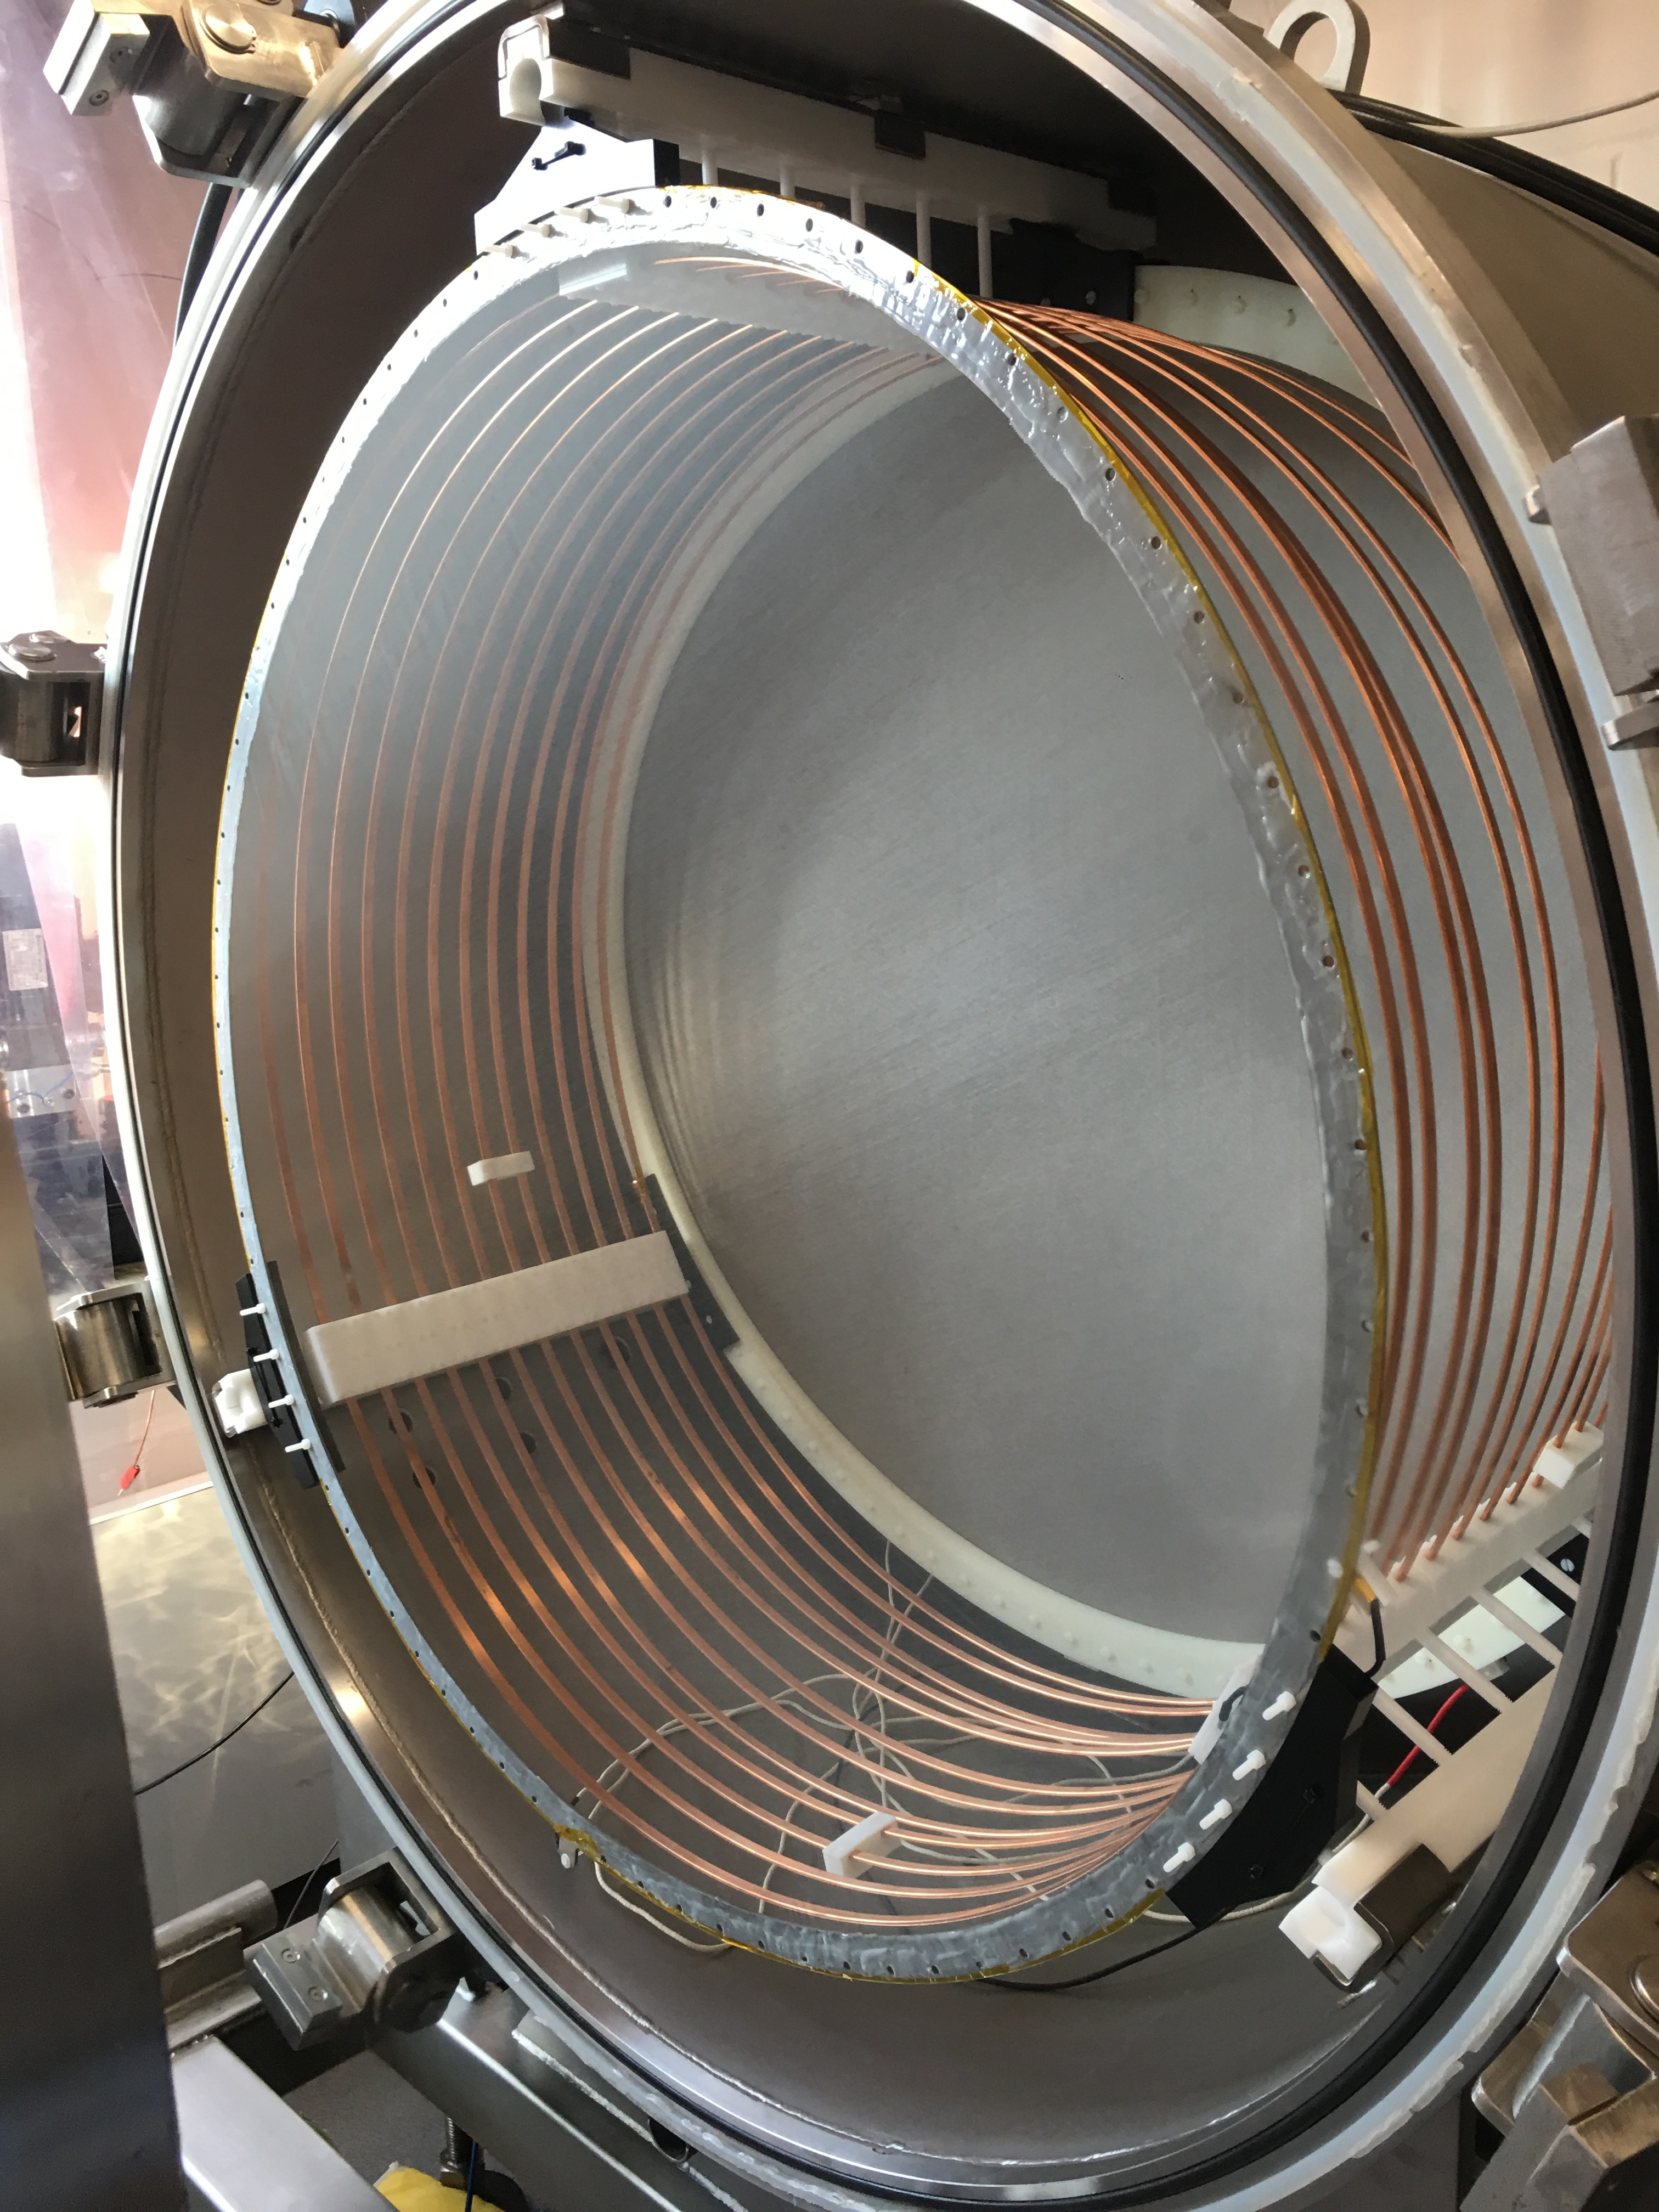
\includegraphics[width=0.6\linewidth]{files/Figures/IMG_1194.jpg}
    	\caption{Cross-sectional view of the TPC; the thing mesh electrodes and copper ring drift volume can be seen inside the steel vessel}
    		\label{fig:TPC}
    \end{figure}
    
    The centre of the TPC was placed 13~m from the beam entrance with S3 and S4 directly upstream and downstream of the vessel, respectively.
    Throughout the run, the TPC was filled with either pure Argon, or a combination of Argon and a small quantity of quencher.
    
	\subsection{Analysis methods -- $S4$}

	Figure~\ref{fig:s4tof} shows the variation in the time of flight spectrum as recorded by $S4$ with a changing number of moderator blocks. 
	This spectrum given by the difference in time between observation of a coincidence in the $S1$ and $S2$ timing points and a signal being recorded in $S4$ (the definition of an $S4$ signal is given above).
	
	\begin{figure}[h]
		\begin{adjustbox}{max totalsize={.8\textwidth}{.7\textheight},center}
			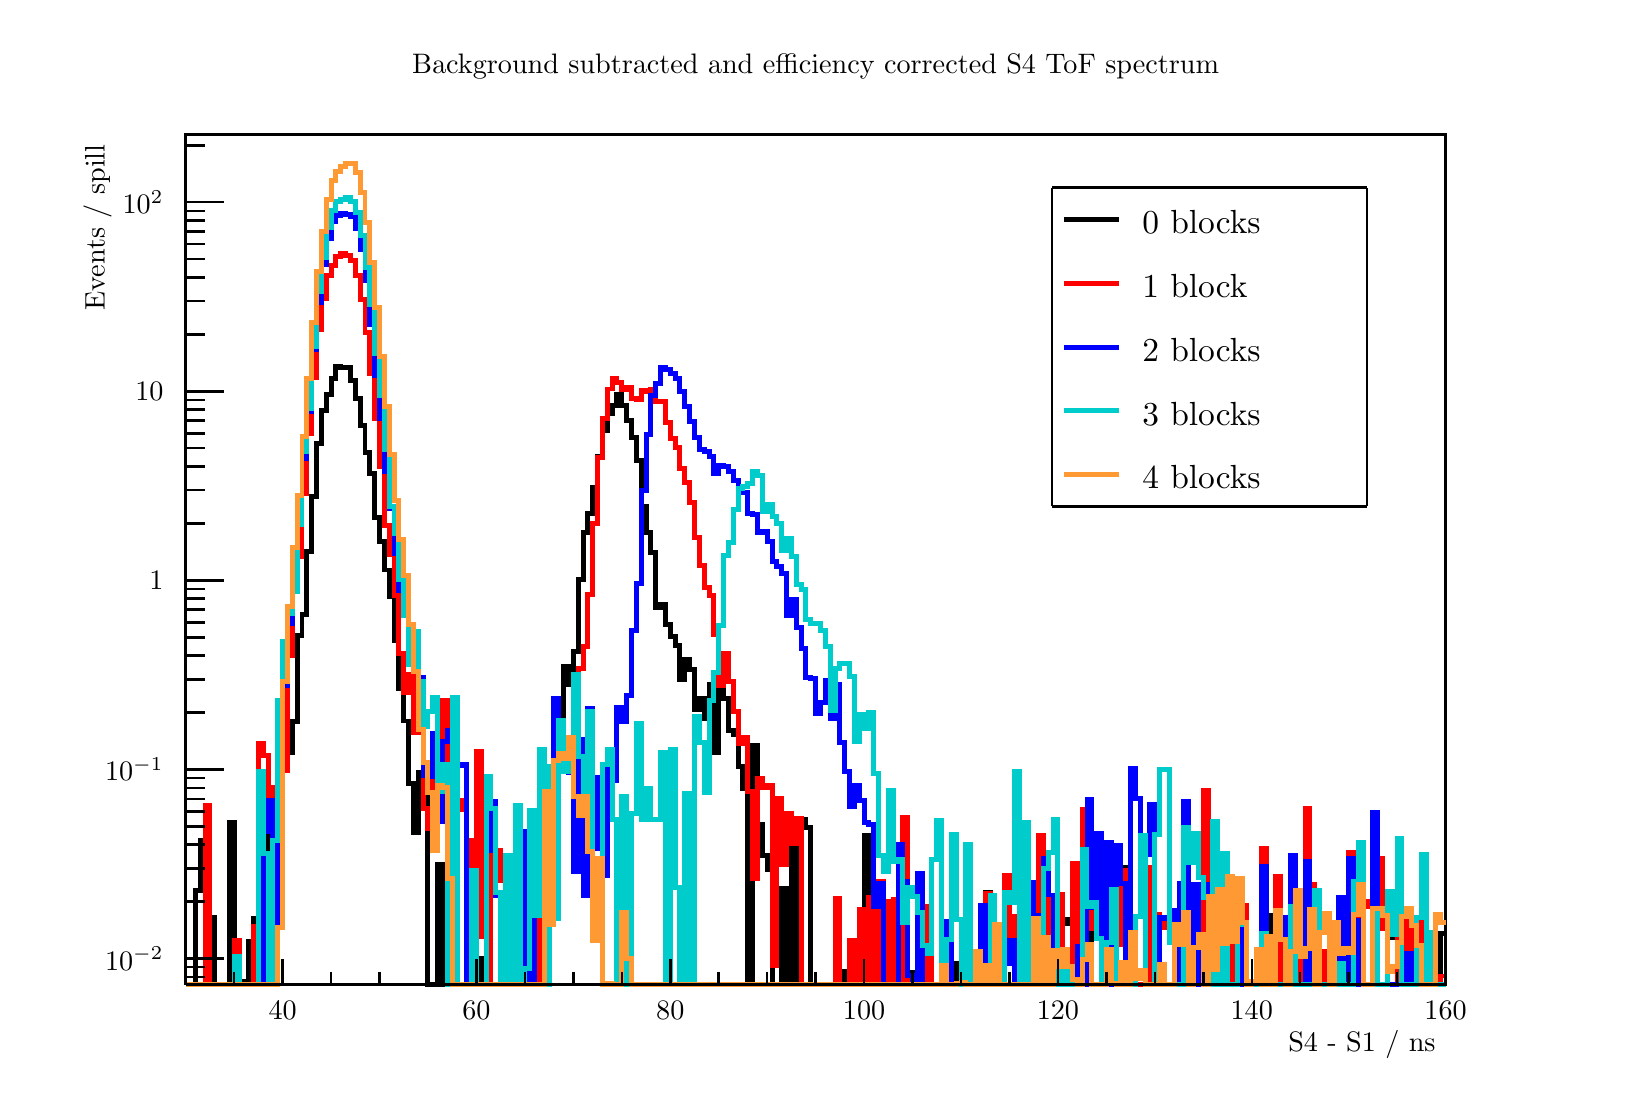
\begin{tikzpicture}
\pgfdeclareplotmark{cross} {
\pgfpathmoveto{\pgfpoint{-0.3\pgfplotmarksize}{\pgfplotmarksize}}
\pgfpathlineto{\pgfpoint{+0.3\pgfplotmarksize}{\pgfplotmarksize}}
\pgfpathlineto{\pgfpoint{+0.3\pgfplotmarksize}{0.3\pgfplotmarksize}}
\pgfpathlineto{\pgfpoint{+1\pgfplotmarksize}{0.3\pgfplotmarksize}}
\pgfpathlineto{\pgfpoint{+1\pgfplotmarksize}{-0.3\pgfplotmarksize}}
\pgfpathlineto{\pgfpoint{+0.3\pgfplotmarksize}{-0.3\pgfplotmarksize}}
\pgfpathlineto{\pgfpoint{+0.3\pgfplotmarksize}{-1.\pgfplotmarksize}}
\pgfpathlineto{\pgfpoint{-0.3\pgfplotmarksize}{-1.\pgfplotmarksize}}
\pgfpathlineto{\pgfpoint{-0.3\pgfplotmarksize}{-0.3\pgfplotmarksize}}
\pgfpathlineto{\pgfpoint{-1.\pgfplotmarksize}{-0.3\pgfplotmarksize}}
\pgfpathlineto{\pgfpoint{-1.\pgfplotmarksize}{0.3\pgfplotmarksize}}
\pgfpathlineto{\pgfpoint{-0.3\pgfplotmarksize}{0.3\pgfplotmarksize}}
\pgfpathclose
\pgfusepathqstroke
}
\pgfdeclareplotmark{cross*} {
\pgfpathmoveto{\pgfpoint{-0.3\pgfplotmarksize}{\pgfplotmarksize}}
\pgfpathlineto{\pgfpoint{+0.3\pgfplotmarksize}{\pgfplotmarksize}}
\pgfpathlineto{\pgfpoint{+0.3\pgfplotmarksize}{0.3\pgfplotmarksize}}
\pgfpathlineto{\pgfpoint{+1\pgfplotmarksize}{0.3\pgfplotmarksize}}
\pgfpathlineto{\pgfpoint{+1\pgfplotmarksize}{-0.3\pgfplotmarksize}}
\pgfpathlineto{\pgfpoint{+0.3\pgfplotmarksize}{-0.3\pgfplotmarksize}}
\pgfpathlineto{\pgfpoint{+0.3\pgfplotmarksize}{-1.\pgfplotmarksize}}
\pgfpathlineto{\pgfpoint{-0.3\pgfplotmarksize}{-1.\pgfplotmarksize}}
\pgfpathlineto{\pgfpoint{-0.3\pgfplotmarksize}{-0.3\pgfplotmarksize}}
\pgfpathlineto{\pgfpoint{-1.\pgfplotmarksize}{-0.3\pgfplotmarksize}}
\pgfpathlineto{\pgfpoint{-1.\pgfplotmarksize}{0.3\pgfplotmarksize}}
\pgfpathlineto{\pgfpoint{-0.3\pgfplotmarksize}{0.3\pgfplotmarksize}}
\pgfpathclose
\pgfusepathqfillstroke
}
\pgfdeclareplotmark{newstar} {
\pgfpathmoveto{\pgfqpoint{0pt}{\pgfplotmarksize}}
\pgfpathlineto{\pgfqpointpolar{44}{0.5\pgfplotmarksize}}
\pgfpathlineto{\pgfqpointpolar{18}{\pgfplotmarksize}}
\pgfpathlineto{\pgfqpointpolar{-20}{0.5\pgfplotmarksize}}
\pgfpathlineto{\pgfqpointpolar{-54}{\pgfplotmarksize}}
\pgfpathlineto{\pgfqpointpolar{-90}{0.5\pgfplotmarksize}}
\pgfpathlineto{\pgfqpointpolar{234}{\pgfplotmarksize}}
\pgfpathlineto{\pgfqpointpolar{198}{0.5\pgfplotmarksize}}
\pgfpathlineto{\pgfqpointpolar{162}{\pgfplotmarksize}}
\pgfpathlineto{\pgfqpointpolar{134}{0.5\pgfplotmarksize}}
\pgfpathclose
\pgfusepathqstroke
}
\pgfdeclareplotmark{newstar*} {
\pgfpathmoveto{\pgfqpoint{0pt}{\pgfplotmarksize}}
\pgfpathlineto{\pgfqpointpolar{44}{0.5\pgfplotmarksize}}
\pgfpathlineto{\pgfqpointpolar{18}{\pgfplotmarksize}}
\pgfpathlineto{\pgfqpointpolar{-20}{0.5\pgfplotmarksize}}
\pgfpathlineto{\pgfqpointpolar{-54}{\pgfplotmarksize}}
\pgfpathlineto{\pgfqpointpolar{-90}{0.5\pgfplotmarksize}}
\pgfpathlineto{\pgfqpointpolar{234}{\pgfplotmarksize}}
\pgfpathlineto{\pgfqpointpolar{198}{0.5\pgfplotmarksize}}
\pgfpathlineto{\pgfqpointpolar{162}{\pgfplotmarksize}}
\pgfpathlineto{\pgfqpointpolar{134}{0.5\pgfplotmarksize}}
\pgfpathclose
\pgfusepathqfillstroke
}
\definecolor{c}{rgb}{1,1,1};
\draw [color=c, fill=c] (0,0) rectangle (20,13.4957);
\draw [color=c, fill=c] (2,1.34957) rectangle (18,12.1461);
\definecolor{c}{rgb}{0,0,0};
\draw [c,line width=0.9] (2,1.34957) -- (2,12.1461) -- (18,12.1461) -- (18,1.34957) -- (2,1.34957);
\definecolor{c}{rgb}{1,1,1};
\draw [color=c, fill=c] (2,1.34957) rectangle (18,12.1461);
\definecolor{c}{rgb}{0,0,0};
\draw [c,line width=0.9] (2,1.34957) -- (2,12.1461) -- (18,12.1461) -- (18,1.34957) -- (2,1.34957);
\definecolor{c}{rgb}{0,0,0.6};
\draw [c,line width=0.9] (2,1.34957) -- (2.06154,1.34957) -- (2.06154,1.34957) -- (2.12308,1.34957) -- (2.12308,1.34957) -- (2.18462,1.34957) -- (2.18462,1.34957) -- (2.24615,1.34957) -- (2.24615,1.34957) -- (2.30769,1.34957) -- (2.30769,1.34957) --
 (2.36923,1.34957) -- (2.36923,1.34957) -- (2.43077,1.34957) -- (2.43077,1.34957) -- (2.49231,1.34957) -- (2.49231,1.34957) -- (2.55385,1.34957) -- (2.55385,1.34957) -- (2.61538,1.34957) -- (2.61538,1.34957) -- (2.67692,1.34957) -- (2.67692,1.34957)
 -- (2.73846,1.34957) -- (2.73846,1.34957) -- (2.8,1.34957) -- (2.8,1.34957) -- (2.86154,1.34957) -- (2.86154,1.34957) -- (2.92308,1.34957) -- (2.92308,1.34957) -- (2.98462,1.34957) -- (2.98462,1.34957) -- (3.04615,1.34957) -- (3.04615,1.34957) --
 (3.10769,1.34957) -- (3.10769,1.34957) -- (3.16923,1.34957) -- (3.16923,1.34957) -- (3.23077,1.34957) -- (3.23077,1.34957) -- (3.29231,1.34957) -- (3.29231,1.34957) -- (3.35385,1.34957) -- (3.35385,1.34957) -- (3.41538,1.34957) -- (3.41538,1.34957)
 -- (3.47692,1.34957) -- (3.47692,1.34957) -- (3.53846,1.34957) -- (3.53846,1.34957) -- (3.6,1.34957) -- (3.6,1.34957) -- (3.66154,1.34957) -- (3.66154,1.34957) -- (3.72308,1.34957) -- (3.72308,1.34957) -- (3.78462,1.34957) -- (3.78462,1.34957) --
 (3.84615,1.34957) -- (3.84615,1.34957) -- (3.90769,1.34957) -- (3.90769,1.34957) -- (3.96923,1.34957) -- (3.96923,1.34957) -- (4.03077,1.34957) -- (4.03077,1.34957) -- (4.09231,1.34957) -- (4.09231,1.34957) -- (4.15385,1.34957) -- (4.15385,1.34957)
 -- (4.21538,1.34957) -- (4.21538,1.34957) -- (4.27692,1.34957) -- (4.27692,1.34957) -- (4.33846,1.34957) -- (4.33846,1.34957) -- (4.4,1.34957) -- (4.4,1.34957) -- (4.46154,1.34957) -- (4.46154,1.34957) -- (4.52308,1.34957) -- (4.52308,1.34957) --
 (4.58462,1.34957) -- (4.58462,1.34957) -- (4.64615,1.34957) -- (4.64615,1.34957) -- (4.70769,1.34957) -- (4.70769,1.34957) -- (4.76923,1.34957) -- (4.76923,1.34957) -- (4.83077,1.34957) -- (4.83077,1.34957) -- (4.89231,1.34957) -- (4.89231,1.34957)
 -- (4.95385,1.34957) -- (4.95385,1.34957) -- (5.01538,1.34957) -- (5.01538,1.34957) -- (5.07692,1.34957) -- (5.07692,1.34957) -- (5.13846,1.34957) -- (5.13846,1.34957) -- (5.2,1.34957) -- (5.2,1.34957) -- (5.26154,1.34957) -- (5.26154,1.34957) --
 (5.32308,1.34957) -- (5.32308,1.34957) -- (5.38462,1.34957) -- (5.38462,1.34957) -- (5.44615,1.34957) -- (5.44615,1.34957) -- (5.50769,1.34957) -- (5.50769,1.34957) -- (5.56923,1.34957) -- (5.56923,1.34957) -- (5.63077,1.34957) -- (5.63077,1.34957)
 -- (5.69231,1.34957) -- (5.69231,1.34957) -- (5.75385,1.34957) -- (5.75385,1.34957) -- (5.81538,1.34957) -- (5.81538,1.34957) -- (5.87692,1.34957) -- (5.87692,1.34957) -- (5.93846,1.34957) -- (5.93846,1.34957) -- (6,1.34957) -- (6,1.34957) --
 (6.06154,1.34957) -- (6.06154,1.34957) -- (6.12308,1.34957) -- (6.12308,1.34957) -- (6.18462,1.34957) -- (6.18462,1.34957) -- (6.24615,1.34957) -- (6.24615,1.34957) -- (6.30769,1.34957) -- (6.30769,1.34957) -- (6.36923,1.34957) -- (6.36923,1.34957)
 -- (6.43077,1.34957) -- (6.43077,1.34957) -- (6.49231,1.34957) -- (6.49231,1.34957) -- (6.55385,1.34957) -- (6.55385,1.34957) -- (6.61538,1.34957) -- (6.61538,1.34957) -- (6.67692,1.34957) -- (6.67692,1.34957) -- (6.73846,1.34957) --
 (6.73846,1.34957) -- (6.8,1.34957) -- (6.8,1.34957) -- (6.86154,1.34957) -- (6.86154,1.34957) -- (6.92308,1.34957) -- (6.92308,1.34957) -- (6.98462,1.34957) -- (6.98462,1.34957) -- (7.04615,1.34957) -- (7.04615,1.34957) -- (7.10769,1.34957) --
 (7.10769,1.34957) -- (7.16923,1.34957) -- (7.16923,1.34957) -- (7.23077,1.34957) -- (7.23077,1.34957) -- (7.29231,1.34957) -- (7.29231,1.34957) -- (7.35385,1.34957) -- (7.35385,1.34957) -- (7.41538,1.34957) -- (7.41538,1.34957) -- (7.47692,1.34957)
 -- (7.47692,1.34957) -- (7.53846,1.34957) -- (7.53846,1.34957) -- (7.6,1.34957) -- (7.6,1.34957) -- (7.66154,1.34957) -- (7.66154,1.34957) -- (7.72308,1.34957) -- (7.72308,1.34957) -- (7.78462,1.34957) -- (7.78462,1.34957) -- (7.84615,1.34957) --
 (7.84615,1.34957) -- (7.90769,1.34957) -- (7.90769,1.34957) -- (7.96923,1.34957) -- (7.96923,1.34957) -- (8.03077,1.34957) -- (8.03077,1.34957) -- (8.09231,1.34957) -- (8.09231,1.34957) -- (8.15385,1.34957) -- (8.15385,1.34957) -- (8.21538,1.34957)
 -- (8.21538,1.34957) -- (8.27692,1.34957) -- (8.27692,1.34957) -- (8.33846,1.34957) -- (8.33846,1.34957) -- (8.4,1.34957) -- (8.4,1.34957) -- (8.46154,1.34957) -- (8.46154,1.34957) -- (8.52308,1.34957) -- (8.52308,1.34957) -- (8.58462,1.34957) --
 (8.58462,1.34957) -- (8.64615,1.34957) -- (8.64615,1.34957) -- (8.70769,1.34957) -- (8.70769,1.34957) -- (8.76923,1.34957) -- (8.76923,1.34957) -- (8.83077,1.34957) -- (8.83077,1.34957) -- (8.89231,1.34957) -- (8.89231,1.34957) -- (8.95385,1.34957)
 -- (8.95385,1.34957) -- (9.01538,1.34957) -- (9.01538,1.34957) -- (9.07692,1.34957) -- (9.07692,1.34957) -- (9.13846,1.34957) -- (9.13846,1.34957) -- (9.2,1.34957) -- (9.2,1.34957) -- (9.26154,1.34957) -- (9.26154,1.34957) -- (9.32308,1.34957) --
 (9.32308,1.34957) -- (9.38461,1.34957) -- (9.38461,1.34957) -- (9.44615,1.34957) -- (9.44615,1.34957) -- (9.50769,1.34957) -- (9.50769,1.34957) -- (9.56923,1.34957) -- (9.56923,1.34957) -- (9.63077,1.34957) -- (9.63077,1.34957) -- (9.69231,1.34957)
 -- (9.69231,1.34957) -- (9.75385,1.34957) -- (9.75385,1.34957) -- (9.81538,1.34957) -- (9.81538,1.34957) -- (9.87692,1.34957) -- (9.87692,1.34957) -- (9.93846,1.34957) -- (9.93846,1.34957) -- (10,1.34957) -- (10,1.34957) -- (10.0615,1.34957) --
 (10.0615,1.34957) -- (10.1231,1.34957) -- (10.1231,1.34957) -- (10.1846,1.34957) -- (10.1846,1.34957) -- (10.2462,1.34957) -- (10.2462,1.34957) -- (10.3077,1.34957) -- (10.3077,1.34957) -- (10.3692,1.34957) -- (10.3692,1.34957) -- (10.4308,1.34957)
 -- (10.4308,1.34957) -- (10.4923,1.34957) -- (10.4923,1.34957) -- (10.5538,1.34957) -- (10.5538,1.34957) -- (10.6154,1.34957) -- (10.6154,1.34957) -- (10.6769,1.34957) -- (10.6769,1.34957) -- (10.7385,1.34957) -- (10.7385,1.34957) -- (10.8,1.34957)
 -- (10.8,1.34957) -- (10.8615,1.34957) -- (10.8615,1.34957) -- (10.9231,1.34957) -- (10.9231,1.34957) -- (10.9846,1.34957) -- (10.9846,1.34957) -- (11.0462,1.34957) -- (11.0462,1.34957) -- (11.1077,1.34957) -- (11.1077,1.34957) -- (11.1692,1.34957)
 -- (11.1692,1.34957) -- (11.2308,1.34957) -- (11.2308,1.34957) -- (11.2923,1.34957) -- (11.2923,1.34957) -- (11.3538,1.34957) -- (11.3538,1.34957) -- (11.4154,1.34957) -- (11.4154,1.34957) -- (11.4769,1.34957) -- (11.4769,1.34957) --
 (11.5385,1.34957) -- (11.5385,1.34957) -- (11.6,1.34957) -- (11.6,1.34957) -- (11.6615,1.34957) -- (11.6615,1.34957) -- (11.7231,1.34957) -- (11.7231,1.34957) -- (11.7846,1.34957) -- (11.7846,1.34957) -- (11.8462,1.34957) -- (11.8462,1.34957) --
 (11.9077,1.34957) -- (11.9077,1.34957) -- (11.9692,1.34957) -- (11.9692,1.34957) -- (12.0308,1.34957) -- (12.0308,1.34957) -- (12.0923,1.34957) -- (12.0923,1.34957) -- (12.1538,1.34957) -- (12.1538,1.34957) -- (12.2154,1.34957) -- (12.2154,1.34957)
 -- (12.2769,1.34957) -- (12.2769,1.34957) -- (12.3385,1.34957) -- (12.3385,1.34957) -- (12.4,1.34957) -- (12.4,1.34957) -- (12.4615,1.34957) -- (12.4615,1.34957) -- (12.5231,1.34957) -- (12.5231,1.34957) -- (12.5846,1.34957) -- (12.5846,1.34957) --
 (12.6462,1.34957) -- (12.6462,1.34957) -- (12.7077,1.34957) -- (12.7077,1.34957) -- (12.7692,1.34957) -- (12.7692,1.34957) -- (12.8308,1.34957) -- (12.8308,1.34957) -- (12.8923,1.34957) -- (12.8923,1.34957) -- (12.9538,1.34957) -- (12.9538,1.34957)
 -- (13.0154,1.34957) -- (13.0154,1.34957) -- (13.0769,1.34957) -- (13.0769,1.34957) -- (13.1385,1.34957) -- (13.1385,1.34957) -- (13.2,1.34957) -- (13.2,1.34957) -- (13.2615,1.34957) -- (13.2615,1.34957) -- (13.3231,1.34957) -- (13.3231,1.34957) --
 (13.3846,1.34957) -- (13.3846,1.34957) -- (13.4462,1.34957) -- (13.4462,1.34957) -- (13.5077,1.34957) -- (13.5077,1.34957) -- (13.5692,1.34957) -- (13.5692,1.34957) -- (13.6308,1.34957) -- (13.6308,1.34957) -- (13.6923,1.34957) -- (13.6923,1.34957)
 -- (13.7538,1.34957) -- (13.7538,1.34957) -- (13.8154,1.34957) -- (13.8154,1.34957) -- (13.8769,1.34957) -- (13.8769,1.34957) -- (13.9385,1.34957) -- (13.9385,1.34957) -- (14,1.34957) -- (14,1.34957) -- (14.0615,1.34957) -- (14.0615,1.34957) --
 (14.1231,1.34957) -- (14.1231,1.34957) -- (14.1846,1.34957) -- (14.1846,1.34957) -- (14.2462,1.34957) -- (14.2462,1.34957) -- (14.3077,1.34957) -- (14.3077,1.34957) -- (14.3692,1.34957) -- (14.3692,1.34957) -- (14.4308,1.34957) -- (14.4308,1.34957)
 -- (14.4923,1.34957) -- (14.4923,1.34957) -- (14.5538,1.34957) -- (14.5538,1.34957) -- (14.6154,1.34957) -- (14.6154,1.34957) -- (14.6769,1.34957) -- (14.6769,1.34957) -- (14.7385,1.34957) -- (14.7385,1.34957) -- (14.8,1.34957) -- (14.8,1.34957) --
 (14.8615,1.34957) -- (14.8615,1.34957) -- (14.9231,1.34957) -- (14.9231,1.34957) -- (14.9846,1.34957) -- (14.9846,1.34957) -- (15.0462,1.34957) -- (15.0462,1.34957) -- (15.1077,1.34957) -- (15.1077,1.34957) -- (15.1692,1.34957) -- (15.1692,1.34957)
 -- (15.2308,1.34957) -- (15.2308,1.34957) -- (15.2923,1.34957) -- (15.2923,1.34957) -- (15.3538,1.34957) -- (15.3538,1.34957) -- (15.4154,1.34957) -- (15.4154,1.34957) -- (15.4769,1.34957) -- (15.4769,1.34957) -- (15.5385,1.34957) --
 (15.5385,1.34957) -- (15.6,1.34957) -- (15.6,1.34957) -- (15.6615,1.34957) -- (15.6615,1.34957) -- (15.7231,1.34957) -- (15.7231,1.34957) -- (15.7846,1.34957) -- (15.7846,1.34957) -- (15.8462,1.34957) -- (15.8462,1.34957) -- (15.9077,1.34957) --
 (15.9077,1.34957) -- (15.9692,1.34957) -- (15.9692,1.34957) -- (16.0308,1.34957) -- (16.0308,1.34957) -- (16.0923,1.34957) -- (16.0923,1.34957) -- (16.1538,1.34957) -- (16.1538,1.34957) -- (16.2154,1.34957) -- (16.2154,1.34957) -- (16.2769,1.34957)
 -- (16.2769,1.34957) -- (16.3385,1.34957) -- (16.3385,1.34957) -- (16.4,1.34957) -- (16.4,1.34957) -- (16.4615,1.34957) -- (16.4615,1.34957) -- (16.5231,1.34957) -- (16.5231,1.34957) -- (16.5846,1.34957) -- (16.5846,1.34957) -- (16.6462,1.34957) --
 (16.6462,1.34957) -- (16.7077,1.34957) -- (16.7077,1.34957) -- (16.7692,1.34957) -- (16.7692,1.34957) -- (16.8308,1.34957) -- (16.8308,1.34957) -- (16.8923,1.34957) -- (16.8923,1.34957) -- (16.9538,1.34957) -- (16.9538,1.34957) -- (17.0154,1.34957)
 -- (17.0154,1.34957) -- (17.0769,1.34957) -- (17.0769,1.34957) -- (17.1385,1.34957) -- (17.1385,1.34957) -- (17.2,1.34957) -- (17.2,1.34957) -- (17.2615,1.34957) -- (17.2615,1.34957) -- (17.3231,1.34957) -- (17.3231,1.34957) -- (17.3846,1.34957) --
 (17.3846,1.34957) -- (17.4462,1.34957) -- (17.4462,1.34957) -- (17.5077,1.34957) -- (17.5077,1.34957) -- (17.5692,1.34957) -- (17.5692,1.34957) -- (17.6308,1.34957) -- (17.6308,1.34957) -- (17.6923,1.34957) -- (17.6923,1.34957) -- (17.7538,1.34957)
 -- (17.7538,1.34957) -- (17.8154,1.34957) -- (17.8154,1.34957) -- (17.8769,1.34957) -- (17.8769,1.34957) -- (17.9385,1.34957) -- (17.9385,1.34957) -- (18,1.34957);
\definecolor{c}{rgb}{0,0,0};
\draw [c,line width=0.9] (2,1.34957) -- (18,1.34957);
\draw [c,line width=0.9] (3.23077,1.67347) -- (3.23077,1.34957);
\draw [c,line width=0.9] (3.84615,1.51152) -- (3.84615,1.34957);
\draw [c,line width=0.9] (4.46154,1.51152) -- (4.46154,1.34957);
\draw [c,line width=0.9] (5.07692,1.51152) -- (5.07692,1.34957);
\draw [c,line width=0.9] (5.69231,1.67347) -- (5.69231,1.34957);
\draw [c,line width=0.9] (6.30769,1.51152) -- (6.30769,1.34957);
\draw [c,line width=0.9] (6.92308,1.51152) -- (6.92308,1.34957);
\draw [c,line width=0.9] (7.53846,1.51152) -- (7.53846,1.34957);
\draw [c,line width=0.9] (8.15385,1.67347) -- (8.15385,1.34957);
\draw [c,line width=0.9] (8.76923,1.51152) -- (8.76923,1.34957);
\draw [c,line width=0.9] (9.38461,1.51152) -- (9.38461,1.34957);
\draw [c,line width=0.9] (10,1.51152) -- (10,1.34957);
\draw [c,line width=0.9] (10.6154,1.67347) -- (10.6154,1.34957);
\draw [c,line width=0.9] (11.2308,1.51152) -- (11.2308,1.34957);
\draw [c,line width=0.9] (11.8462,1.51152) -- (11.8462,1.34957);
\draw [c,line width=0.9] (12.4615,1.51152) -- (12.4615,1.34957);
\draw [c,line width=0.9] (13.0769,1.67347) -- (13.0769,1.34957);
\draw [c,line width=0.9] (13.6923,1.51152) -- (13.6923,1.34957);
\draw [c,line width=0.9] (14.3077,1.51152) -- (14.3077,1.34957);
\draw [c,line width=0.9] (14.9231,1.51152) -- (14.9231,1.34957);
\draw [c,line width=0.9] (15.5385,1.67347) -- (15.5385,1.34957);
\draw [c,line width=0.9] (16.1538,1.51152) -- (16.1538,1.34957);
\draw [c,line width=0.9] (16.7692,1.51152) -- (16.7692,1.34957);
\draw [c,line width=0.9] (17.3846,1.51152) -- (17.3846,1.34957);
\draw [c,line width=0.9] (18,1.67347) -- (18,1.34957);
\draw [c,line width=0.9] (3.23077,1.67347) -- (3.23077,1.34957);
\draw [c,line width=0.9] (2.61538,1.51152) -- (2.61538,1.34957);
\draw [c,line width=0.9] (2,1.51152) -- (2,1.34957);
\draw [anchor=base] (3.23077,0.904212) node[scale=1.01821, color=c, rotate=0]{40};
\draw [anchor=base] (5.69231,0.904212) node[scale=1.01821, color=c, rotate=0]{60};
\draw [anchor=base] (8.15385,0.904212) node[scale=1.01821, color=c, rotate=0]{80};
\draw [anchor=base] (10.6154,0.904212) node[scale=1.01821, color=c, rotate=0]{100};
\draw [anchor=base] (13.0769,0.904212) node[scale=1.01821, color=c, rotate=0]{120};
\draw [anchor=base] (15.5385,0.904212) node[scale=1.01821, color=c, rotate=0]{140};
\draw [anchor=base] (18,0.904212) node[scale=1.01821, color=c, rotate=0]{160};
\draw [anchor= east] (18,0.593811) node[scale=1.01821, color=c, rotate=0]{ S4 - S1 / ns};
\draw [c,line width=0.9] (2,1.34957) -- (2,12.1461);
\draw [c,line width=0.9] (2.24,1.44788) -- (2,1.44788);
\draw [c,line width=0.9] (2.24,1.57071) -- (2,1.57071);
\draw [c,line width=0.9] (2.48,1.68059) -- (2,1.68059);
\draw [anchor= east] (1.844,1.68059) node[scale=1.01821, color=c, rotate=0]{$10^{-2}$};
\draw [c,line width=0.9] (2.24,2.40344) -- (2,2.40344);
\draw [c,line width=0.9] (2.24,2.82629) -- (2,2.82629);
\draw [c,line width=0.9] (2.24,3.1263) -- (2,3.1263);
\draw [c,line width=0.9] (2.24,3.35901) -- (2,3.35901);
\draw [c,line width=0.9] (2.24,3.54914) -- (2,3.54914);
\draw [c,line width=0.9] (2.24,3.7099) -- (2,3.7099);
\draw [c,line width=0.9] (2.24,3.84916) -- (2,3.84916);
\draw [c,line width=0.9] (2.24,3.97199) -- (2,3.97199);
\draw [c,line width=0.9] (2.48,4.08186) -- (2,4.08186);
\draw [anchor= east] (1.844,4.08186) node[scale=1.01821, color=c, rotate=0]{$10^{-1}$};
\draw [c,line width=0.9] (2.24,4.80472) -- (2,4.80472);
\draw [c,line width=0.9] (2.24,5.22756) -- (2,5.22756);
\draw [c,line width=0.9] (2.24,5.52758) -- (2,5.52758);
\draw [c,line width=0.9] (2.24,5.76028) -- (2,5.76028);
\draw [c,line width=0.9] (2.24,5.95042) -- (2,5.95042);
\draw [c,line width=0.9] (2.24,6.11118) -- (2,6.11118);
\draw [c,line width=0.9] (2.24,6.25043) -- (2,6.25043);
\draw [c,line width=0.9] (2.24,6.37327) -- (2,6.37327);
\draw [c,line width=0.9] (2.48,6.48314) -- (2,6.48314);
\draw [anchor= east] (1.844,6.48314) node[scale=1.01821, color=c, rotate=0]{1};
\draw [c,line width=0.9] (2.24,7.206) -- (2,7.206);
\draw [c,line width=0.9] (2.24,7.62884) -- (2,7.62884);
\draw [c,line width=0.9] (2.24,7.92885) -- (2,7.92885);
\draw [c,line width=0.9] (2.24,8.16156) -- (2,8.16156);
\draw [c,line width=0.9] (2.24,8.3517) -- (2,8.3517);
\draw [c,line width=0.9] (2.24,8.51246) -- (2,8.51246);
\draw [c,line width=0.9] (2.24,8.65171) -- (2,8.65171);
\draw [c,line width=0.9] (2.24,8.77454) -- (2,8.77454);
\draw [c,line width=0.9] (2.48,8.88442) -- (2,8.88442);
\draw [anchor= east] (1.844,8.88442) node[scale=1.01821, color=c, rotate=0]{10};
\draw [c,line width=0.9] (2.24,9.60728) -- (2,9.60728);
\draw [c,line width=0.9] (2.24,10.0301) -- (2,10.0301);
\draw [c,line width=0.9] (2.24,10.3301) -- (2,10.3301);
\draw [c,line width=0.9] (2.24,10.5628) -- (2,10.5628);
\draw [c,line width=0.9] (2.24,10.753) -- (2,10.753);
\draw [c,line width=0.9] (2.24,10.9137) -- (2,10.9137);
\draw [c,line width=0.9] (2.24,11.053) -- (2,11.053);
\draw [c,line width=0.9] (2.24,11.1758) -- (2,11.1758);
\draw [c,line width=0.9] (2.48,11.2857) -- (2,11.2857);
\draw [anchor= east] (1.844,11.2857) node[scale=1.01821, color=c, rotate=0]{$10^{2}$};
\draw [c,line width=0.9] (2.24,12.0086) -- (2,12.0086);
\draw [anchor= east] (0.88,12.1461) node[scale=1.01821, color=c, rotate=90]{ Events / spill};
\draw [c,line width=1.8] (2,1.34957) -- (2.06154,1.34957) -- (2.06154,1.34957) -- (2.12308,1.34957) -- (2.12308,2.53951) -- (2.18462,2.53951) -- (2.18462,3.17729) -- (2.24615,3.17729) -- (2.24615,1.34957) -- (2.30769,1.34957) -- (2.30769,2.20144) --
 (2.36923,2.20144) -- (2.36923,1.34957) -- (2.43077,1.34957) -- (2.43077,1.34957) -- (2.49231,1.34957) -- (2.49231,1.34957) -- (2.55385,1.34957) -- (2.55385,3.40479) -- (2.61538,3.40479) -- (2.61538,1.34957) -- (2.67692,1.34957) -- (2.67692,1.34957)
 -- (2.73846,1.34957) -- (2.73846,1.38687) -- (2.8,1.38687) -- (2.8,1.90133) -- (2.86154,1.90133) -- (2.86154,2.18515) -- (2.92308,2.18515) -- (2.92308,3.61789) -- (2.98462,3.61789) -- (2.98462,3.25403) -- (3.04615,3.25403) -- (3.04615,1.34957) --
 (3.10769,1.34957) -- (3.10769,3.39189) -- (3.16923,3.39189) -- (3.16923,4.13184) -- (3.23077,4.13184) -- (3.23077,4.44884) -- (3.29231,4.44884) -- (3.29231,4.30025) -- (3.35385,4.30025) -- (3.35385,4.68859) -- (3.41538,4.68859) -- (3.41538,5.78092)
 -- (3.47692,5.78092) -- (3.47692,6.05252) -- (3.53846,6.05252) -- (3.53846,6.85477) -- (3.6,6.85477) -- (3.6,7.55269) -- (3.66154,7.55269) -- (3.66154,8.22225) -- (3.72308,8.22225) -- (3.72308,8.64481) -- (3.78462,8.64481) -- (3.78462,8.84179) --
 (3.84615,8.84179) -- (3.84615,9.04392) -- (3.90769,9.04392) -- (3.90769,9.20268) -- (3.96923,9.20268) -- (3.96923,9.18123) -- (4.03077,9.18123) -- (4.03077,9.19048) -- (4.09231,9.19048) -- (4.09231,9.02681) -- (4.15385,9.02681) -- (4.15385,8.78913)
 -- (4.21538,8.78913) -- (4.21538,8.45125) -- (4.27692,8.45125) -- (4.27692,8.10572) -- (4.33846,8.10572) -- (4.33846,7.84076) -- (4.4,7.84076) -- (4.4,7.28435) -- (4.46154,7.28435) -- (4.46154,6.98214) -- (4.52308,6.98214) -- (4.52308,6.61504) --
 (4.58462,6.61504) -- (4.58462,6.27553) -- (4.64615,6.27553) -- (4.64615,5.72202) -- (4.70769,5.72202) -- (4.70769,5.11195) -- (4.76923,5.11195) -- (4.76923,4.69735) -- (4.83077,4.69735) -- (4.83077,3.90316) -- (4.89231,3.90316) -- (4.89231,3.28257)
 -- (4.95385,3.28257) -- (4.95385,4.04247) -- (5.01538,4.04247) -- (5.01538,3.738) -- (5.07692,3.738) -- (5.07692,1.34957) -- (5.13846,1.34957) -- (5.13846,1.34957) -- (5.2,1.34957) -- (5.2,2.87862) -- (5.26154,2.87862) -- (5.26154,1.34957) --
 (5.32308,1.34957) -- (5.32308,2.92743) -- (5.38462,2.92743) -- (5.38462,3.00257) -- (5.44615,3.00257) -- (5.44615,1.34957) -- (5.50769,1.34957) -- (5.50769,1.34957) -- (5.56923,1.34957) -- (5.56923,1.34957) -- (5.63077,1.34957) -- (5.63077,1.34957)
 -- (5.69231,1.34957) -- (5.69231,1.68015) -- (5.75385,1.68015) -- (5.75385,1.34957) -- (5.81538,1.34957) -- (5.81538,2.57343) -- (5.87692,2.57343) -- (5.87692,1.34957) -- (5.93846,1.34957) -- (5.93846,1.34957) -- (6,1.34957) -- (6,1.34957) --
 (6.06154,1.34957) -- (6.06154,1.34957) -- (6.12308,1.34957) -- (6.12308,1.34957) -- (6.18462,1.34957) -- (6.18462,1.34957) -- (6.24615,1.34957) -- (6.24615,2.06003) -- (6.30769,2.06003) -- (6.30769,1.34957) -- (6.36923,1.34957) -- (6.36923,1.34957)
 -- (6.43077,1.34957) -- (6.43077,3.20391) -- (6.49231,3.20391) -- (6.49231,2.17723) -- (6.55385,2.17723) -- (6.55385,3.12456) -- (6.61538,3.12456) -- (6.61538,3.55551) -- (6.67692,3.55551) -- (6.67692,4.3017) -- (6.73846,4.3017) -- (6.73846,4.53853)
 -- (6.8,4.53853) -- (6.8,5.38926) -- (6.86154,5.38926) -- (6.86154,5.16006) -- (6.92308,5.16006) -- (6.92308,5.57801) -- (6.98462,5.57801) -- (6.98462,6.49955) -- (7.04615,6.49955) -- (7.04615,7.08983) -- (7.10769,7.08983) -- (7.10769,7.32942) --
 (7.16923,7.32942) -- (7.16923,7.66242) -- (7.23077,7.66242) -- (7.23077,8.06249) -- (7.29231,8.06249) -- (7.29231,8.38303) -- (7.35385,8.38303) -- (7.35385,8.60368) -- (7.41538,8.60368) -- (7.41538,8.70027) -- (7.47692,8.70027) -- (7.47692,8.84394)
 -- (7.53846,8.84394) -- (7.53846,8.70221) -- (7.6,8.70221) -- (7.6,8.51775) -- (7.66154,8.51775) -- (7.66154,8.29905) -- (7.72308,8.29905) -- (7.72308,8.00204) -- (7.78462,8.00204) -- (7.78462,7.42284) -- (7.84615,7.42284) -- (7.84615,7.09375) --
 (7.90769,7.09375) -- (7.90769,6.83915) -- (7.96923,6.83915) -- (7.96923,6.1409) -- (8.03077,6.1409) -- (8.03077,6.18103) -- (8.09231,6.18103) -- (8.09231,5.92597) -- (8.15385,5.92597) -- (8.15385,5.76712) -- (8.21538,5.76712) -- (8.21538,5.6565) --
 (8.27692,5.6565) -- (8.27692,5.2214) -- (8.33846,5.2214) -- (8.33846,5.48398) -- (8.4,5.48398) -- (8.4,5.35061) -- (8.46154,5.35061) -- (8.46154,4.83908) -- (8.52308,4.83908) -- (8.52308,4.97696) -- (8.58462,4.97696) -- (8.58462,4.72547) --
 (8.64615,4.72547) -- (8.64615,5.16273) -- (8.70769,5.16273) -- (8.70769,4.30101) -- (8.76923,4.30101) -- (8.76923,5.1798) -- (8.83077,5.1798) -- (8.83077,4.98008) -- (8.89231,4.98008) -- (8.89231,4.57223) -- (8.95385,4.57223) -- (8.95385,4.52429) --
 (9.01538,4.52429) -- (9.01538,4.11848) -- (9.07692,4.11848) -- (9.07692,3.84027) -- (9.13846,3.84027) -- (9.13846,1.34957) -- (9.2,1.34957) -- (9.2,4.38175) -- (9.26154,4.38175) -- (9.26154,3.37945) -- (9.32308,3.37945) -- (9.32308,2.98425) --
 (9.38461,2.98425) -- (9.38461,2.81682) -- (9.44615,2.81682) -- (9.44615,1.34957) -- (9.50769,1.34957) -- (9.50769,1.34957) -- (9.56923,1.34957) -- (9.56923,2.56799) -- (9.63077,2.56799) -- (9.63077,1.34957) -- (9.69231,1.34957) -- (9.69231,3.38931)
 -- (9.75385,3.38931) -- (9.75385,1.34957) -- (9.81538,1.34957) -- (9.81538,3.44534) -- (9.87692,3.44534) -- (9.87692,3.34676) -- (9.93846,3.34676) -- (9.93846,1.34957) -- (10,1.34957) -- (10,1.34957) -- (10.0615,1.34957) -- (10.0615,1.34957) --
 (10.1231,1.34957) -- (10.1231,1.34957) -- (10.1846,1.34957) -- (10.1846,1.34957) -- (10.2462,1.34957) -- (10.2462,1.34957) -- (10.3077,1.34957) -- (10.3077,1.51017) -- (10.3692,1.51017) -- (10.3692,1.34957) -- (10.4308,1.34957) -- (10.4308,1.34957)
 -- (10.4923,1.34957) -- (10.4923,1.34957) -- (10.5538,1.34957) -- (10.5538,1.34957) -- (10.6154,1.34957) -- (10.6154,3.2483) -- (10.6769,3.2483) -- (10.6769,1.77041) -- (10.7385,1.77041) -- (10.7385,1.34957) -- (10.8,1.34957) -- (10.8,1.34957) --
 (10.8615,1.34957) -- (10.8615,1.34957) -- (10.9231,1.34957) -- (10.9231,1.34957) -- (10.9846,1.34957) -- (10.9846,1.34957) -- (11.0462,1.34957) -- (11.0462,1.34957) -- (11.1077,1.34957) -- (11.1077,1.34957) -- (11.1692,1.34957) -- (11.1692,1.49969)
 -- (11.2308,1.49969) -- (11.2308,1.34957) -- (11.2923,1.34957) -- (11.2923,1.34957) -- (11.3538,1.34957) -- (11.3538,1.34957) -- (11.4154,1.34957) -- (11.4154,1.34957) -- (11.4769,1.34957) -- (11.4769,1.34957) -- (11.5385,1.34957) --
 (11.5385,1.34957) -- (11.6,1.34957) -- (11.6,1.34957) -- (11.6615,1.34957) -- (11.6615,1.85741) -- (11.7231,1.85741) -- (11.7231,1.34957) -- (11.7846,1.34957) -- (11.7846,1.62176) -- (11.8462,1.62176) -- (11.8462,1.34957) -- (11.9077,1.34957) --
 (11.9077,1.34957) -- (11.9692,1.34957) -- (11.9692,1.35861) -- (12.0308,1.35861) -- (12.0308,1.34957) -- (12.0923,1.34957) -- (12.0923,1.34957) -- (12.1538,1.34957) -- (12.1538,2.52198) -- (12.2154,2.52198) -- (12.2154,1.34957) -- (12.2769,1.34957)
 -- (12.2769,1.34957) -- (12.3385,1.34957) -- (12.3385,1.34957) -- (12.4,1.34957) -- (12.4,1.34957) -- (12.4615,1.34957) -- (12.4615,1.34957) -- (12.5231,1.34957) -- (12.5231,1.78978) -- (12.5846,1.78978) -- (12.5846,1.34957) -- (12.6462,1.34957) --
 (12.6462,1.34957) -- (12.7077,1.34957) -- (12.7077,1.34957) -- (12.7692,1.34957) -- (12.7692,1.34957) -- (12.8308,1.34957) -- (12.8308,1.34957) -- (12.8923,1.34957) -- (12.8923,2.1804) -- (12.9538,2.1804) -- (12.9538,1.34957) -- (13.0154,1.34957) --
 (13.0154,1.34957) -- (13.0769,1.34957) -- (13.0769,1.34957) -- (13.1385,1.34957) -- (13.1385,2.1314) -- (13.2,2.1314) -- (13.2,2.1798) -- (13.2615,2.1798) -- (13.2615,1.34957) -- (13.3231,1.34957) -- (13.3231,1.34957) -- (13.3846,1.34957) --
 (13.3846,1.34957) -- (13.4462,1.34957) -- (13.4462,1.34957) -- (13.5077,1.34957) -- (13.5077,2.64658) -- (13.5692,2.64658) -- (13.5692,2.39108) -- (13.6308,2.39108) -- (13.6308,1.34957) -- (13.6923,1.34957) -- (13.6923,1.34957) -- (13.7538,1.34957)
 -- (13.7538,1.34957) -- (13.8154,1.34957) -- (13.8154,1.34957) -- (13.8769,1.34957) -- (13.8769,1.34957) -- (13.9385,1.34957) -- (13.9385,2.83893) -- (14,2.83893) -- (14,2.11491) -- (14.0615,2.11491) -- (14.0615,1.34957) -- (14.1231,1.34957) --
 (14.1231,1.34957) -- (14.1846,1.34957) -- (14.1846,1.34957) -- (14.2462,1.34957) -- (14.2462,1.34957) -- (14.3077,1.34957) -- (14.3077,1.76693) -- (14.3692,1.76693) -- (14.3692,1.34957) -- (14.4308,1.34957) -- (14.4308,1.34957) -- (14.4923,1.34957)
 -- (14.4923,1.34957) -- (14.5538,1.34957) -- (14.5538,1.34957) -- (14.6154,1.34957) -- (14.6154,1.34957) -- (14.6769,1.34957) -- (14.6769,1.34957) -- (14.7385,1.34957) -- (14.7385,2.3037) -- (14.8,2.3037) -- (14.8,1.34957) -- (14.8615,1.34957) --
 (14.8615,1.34957) -- (14.9231,1.34957) -- (14.9231,1.34957) -- (14.9846,1.34957) -- (14.9846,1.34957) -- (15.0462,1.34957) -- (15.0462,1.34957) -- (15.1077,1.34957) -- (15.1077,1.34957) -- (15.1692,1.34957) -- (15.1692,1.34957) -- (15.2308,1.34957)
 -- (15.2308,1.34957) -- (15.2923,1.34957) -- (15.2923,2.5842) -- (15.3538,2.5842) -- (15.3538,1.34957) -- (15.4154,1.34957) -- (15.4154,1.34957) -- (15.4769,1.34957) -- (15.4769,1.34957) -- (15.5385,1.34957) -- (15.5385,1.34957) -- (15.6,1.34957) --
 (15.6,1.34957) -- (15.6615,1.34957) -- (15.6615,1.34957) -- (15.7231,1.34957) -- (15.7231,1.34957) -- (15.7846,1.34957) -- (15.7846,2.22124) -- (15.8462,2.22124) -- (15.8462,1.34957) -- (15.9077,1.34957) -- (15.9077,1.95528) -- (15.9692,1.95528) --
 (15.9692,1.34957) -- (16.0308,1.34957) -- (16.0308,1.34957) -- (16.0923,1.34957) -- (16.0923,1.34957) -- (16.1538,1.34957) -- (16.1538,1.34957) -- (16.2154,1.34957) -- (16.2154,1.34957) -- (16.2769,1.34957) -- (16.2769,1.34957) -- (16.3385,1.34957)
 -- (16.3385,1.34957) -- (16.4,1.34957) -- (16.4,1.34957) -- (16.4615,1.34957) -- (16.4615,1.34957) -- (16.5231,1.34957) -- (16.5231,1.34957) -- (16.5846,1.34957) -- (16.5846,1.34957) -- (16.6462,1.34957) -- (16.6462,1.34957) -- (16.7077,1.34957) --
 (16.7077,1.34957) -- (16.7692,1.34957) -- (16.7692,1.34957) -- (16.8308,1.34957) -- (16.8308,1.34957) -- (16.8923,1.34957) -- (16.8923,1.34957) -- (16.9538,1.34957) -- (16.9538,1.34957) -- (17.0154,1.34957) -- (17.0154,1.34957) -- (17.0769,1.34957)
 -- (17.0769,1.34957) -- (17.1385,1.34957) -- (17.1385,1.34957) -- (17.2,1.34957) -- (17.2,1.34957) -- (17.2615,1.34957) -- (17.2615,1.95386) -- (17.3231,1.95386) -- (17.3231,2.36022) -- (17.3846,2.36022) -- (17.3846,1.34957) -- (17.4462,1.34957) --
 (17.4462,1.34957) -- (17.5077,1.34957) -- (17.5077,1.34957) -- (17.5692,1.34957) -- (17.5692,1.34957) -- (17.6308,1.34957) -- (17.6308,1.34957) -- (17.6923,1.34957) -- (17.6923,1.34957) -- (17.7538,1.34957) -- (17.7538,1.34957) -- (17.8154,1.34957)
 -- (17.8154,1.34957) -- (17.8769,1.34957) -- (17.8769,1.34957) -- (17.9385,1.34957) -- (17.9385,1.99545) -- (18,1.99545);
\definecolor{c}{rgb}{1,0,0};
\draw [c,line width=1.8] (2,1.34957) -- (2.06154,1.34957) -- (2.06154,1.34957) -- (2.12308,1.34957) -- (2.12308,1.34957) -- (2.18462,1.34957) -- (2.18462,1.34957) -- (2.24615,1.34957) -- (2.24615,3.62161) -- (2.30769,3.62161) -- (2.30769,1.34957) --
 (2.36923,1.34957) -- (2.36923,1.34957) -- (2.43077,1.34957) -- (2.43077,1.34957) -- (2.49231,1.34957) -- (2.49231,1.34957) -- (2.55385,1.34957) -- (2.55385,1.34957) -- (2.61538,1.34957) -- (2.61538,1.91584) -- (2.67692,1.91584) -- (2.67692,1.34957)
 -- (2.73846,1.34957) -- (2.73846,1.34957) -- (2.8,1.34957) -- (2.8,1.34957) -- (2.86154,1.34957) -- (2.86154,2.08919) -- (2.92308,2.08919) -- (2.92308,4.4145) -- (2.98462,4.4145) -- (2.98462,4.26301) -- (3.04615,4.26301) -- (3.04615,3.61527) --
 (3.10769,3.61527) -- (3.10769,3.85244) -- (3.16923,3.85244) -- (3.16923,4.38046) -- (3.23077,4.38046) -- (3.23077,4.07497) -- (3.29231,4.07497) -- (3.29231,5.53218) -- (3.35385,5.53218) -- (3.35385,6.47699) -- (3.41538,6.47699) -- (3.41538,6.78566)
 -- (3.47692,6.78566) -- (3.47692,7.59064) -- (3.53846,7.59064) -- (3.53846,8.35131) -- (3.6,8.35131) -- (3.6,9.06486) -- (3.66154,9.06486) -- (3.66154,9.66563) -- (3.72308,9.66563) -- (3.72308,10.0693) -- (3.78462,10.0693) -- (3.78462,10.3609) --
 (3.84615,10.3609) -- (3.84615,10.4829) -- (3.90769,10.4829) -- (3.90769,10.5931) -- (3.96923,10.5931) -- (3.96923,10.6313) -- (4.03077,10.6313) -- (4.03077,10.6118) -- (4.09231,10.6118) -- (4.09231,10.5475) -- (4.15385,10.5475) -- (4.15385,10.3521)
 -- (4.21538,10.3521) -- (4.21538,10.0547) -- (4.27692,10.0547) -- (4.27692,9.63751) -- (4.33846,9.63751) -- (4.33846,9.11073) -- (4.4,9.11073) -- (4.4,8.53346) -- (4.46154,8.53346) -- (4.46154,7.93332) -- (4.52308,7.93332) -- (4.52308,7.18344) --
 (4.58462,7.18344) -- (4.58462,6.81416) -- (4.64615,6.81416) -- (4.64615,6.29079) -- (4.70769,6.29079) -- (4.70769,5.55098) -- (4.76923,5.55098) -- (4.76923,5.06016) -- (4.83077,5.06016) -- (4.83077,5.28237) -- (4.89231,5.28237) -- (4.89231,4.54614)
 -- (4.95385,4.54614) -- (4.95385,4.60508) -- (5.01538,4.60508) -- (5.01538,3.59119) -- (5.07692,3.59119) -- (5.07692,3.33771) -- (5.13846,3.33771) -- (5.13846,4.31041) -- (5.2,4.31041) -- (5.2,4.02115) -- (5.26154,4.02115) -- (5.26154,4.96132) --
 (5.32308,4.96132) -- (5.32308,3.64012) -- (5.38462,3.64012) -- (5.38462,3.17982) -- (5.44615,3.17982) -- (5.44615,3.57534) -- (5.50769,3.57534) -- (5.50769,3.68747) -- (5.56923,3.68747) -- (5.56923,3.18227) -- (5.63077,3.18227) -- (5.63077,1.34957)
 -- (5.69231,1.34957) -- (5.69231,4.30999) -- (5.75385,4.30999) -- (5.75385,1.95629) -- (5.81538,1.95629) -- (5.81538,1.34957) -- (5.87692,1.34957) -- (5.87692,3.12297) -- (5.93846,3.12297) -- (5.93846,3.05309) -- (6,3.05309) -- (6,2.6762) --
 (6.06154,2.6762) -- (6.06154,2.30519) -- (6.12308,2.30519) -- (6.12308,1.80391) -- (6.18462,1.80391) -- (6.18462,2.48112) -- (6.24615,2.48112) -- (6.24615,1.34957) -- (6.30769,1.34957) -- (6.30769,1.34957) -- (6.36923,1.34957) -- (6.36923,1.34957)
 -- (6.43077,1.34957) -- (6.43077,1.34957) -- (6.49231,1.34957) -- (6.49231,3.16213) -- (6.55385,3.16213) -- (6.55385,2.75945) -- (6.61538,2.75945) -- (6.61538,4.00308) -- (6.67692,4.00308) -- (6.67692,4.33309) -- (6.73846,4.33309) --
 (6.73846,4.39393) -- (6.8,4.39393) -- (6.8,4.21582) -- (6.86154,4.21582) -- (6.86154,4.19149) -- (6.92308,4.19149) -- (6.92308,4.95959) -- (6.98462,4.95959) -- (6.98462,5.36654) -- (7.04615,5.36654) -- (7.04615,5.64098) -- (7.10769,5.64098) --
 (7.10769,6.29884) -- (7.16923,6.29884) -- (7.16923,7.20416) -- (7.23077,7.20416) -- (7.23077,8.04797) -- (7.29231,8.04797) -- (7.29231,8.54071) -- (7.35385,8.54071) -- (7.35385,8.91385) -- (7.41538,8.91385) -- (7.41538,9.04707) -- (7.47692,9.04707)
 -- (7.47692,8.99555) -- (7.53846,8.99555) -- (7.53846,8.90349) -- (7.6,8.90349) -- (7.6,8.93229) -- (7.66154,8.93229) -- (7.66154,8.79037) -- (7.72308,8.79037) -- (7.72308,8.77626) -- (7.78462,8.77626) -- (7.78462,8.89617) -- (7.84615,8.89617) --
 (7.84615,8.87567) -- (7.90769,8.87567) -- (7.90769,8.90707) -- (7.96923,8.90707) -- (7.96923,8.75828) -- (8.03077,8.75828) -- (8.03077,8.74976) -- (8.09231,8.74976) -- (8.09231,8.48745) -- (8.15385,8.48745) -- (8.15385,8.28347) -- (8.21538,8.28347)
 -- (8.21538,8.1741) -- (8.27692,8.1741) -- (8.27692,7.90876) -- (8.33846,7.90876) -- (8.33846,7.7225) -- (8.4,7.7225) -- (8.4,7.47768) -- (8.46154,7.47768) -- (8.46154,7.03069) -- (8.52308,7.03069) -- (8.52308,6.67147) -- (8.58462,6.67147) --
 (8.58462,6.39729) -- (8.64615,6.39729) -- (8.64615,6.29457) -- (8.70769,6.29457) -- (8.70769,5.80017) -- (8.76923,5.80017) -- (8.76923,5.15044) -- (8.83077,5.15044) -- (8.83077,5.55743) -- (8.89231,5.55743) -- (8.89231,5.20087) -- (8.95385,5.20087)
 -- (8.95385,4.81439) -- (9.01538,4.81439) -- (9.01538,4.40663) -- (9.07692,4.40663) -- (9.07692,4.48419) -- (9.13846,4.48419) -- (9.13846,3.80072) -- (9.2,3.80072) -- (9.2,2.70315) -- (9.26154,2.70315) -- (9.26154,3.96834) -- (9.32308,3.96834) --
 (9.32308,3.84722) -- (9.38461,3.84722) -- (9.38461,3.8737) -- (9.44615,3.8737) -- (9.44615,1.59699) -- (9.50769,1.59699) -- (9.50769,3.71748) -- (9.56923,3.71748) -- (9.56923,2.87557) -- (9.63077,2.87557) -- (9.63077,3.52477) -- (9.69231,3.52477) --
 (9.69231,3.1478) -- (9.75385,3.1478) -- (9.75385,3.46079) -- (9.81538,3.46079) -- (9.81538,1.34957) -- (9.87692,1.34957) -- (9.87692,1.34957) -- (9.93846,1.34957) -- (9.93846,1.34957) -- (10,1.34957) -- (10,1.34957) -- (10.0615,1.34957) --
 (10.0615,1.34957) -- (10.1231,1.34957) -- (10.1231,1.34957) -- (10.1846,1.34957) -- (10.1846,1.34957) -- (10.2462,1.34957) -- (10.2462,2.44947) -- (10.3077,2.44947) -- (10.3077,1.34957) -- (10.3692,1.34957) -- (10.3692,1.34957) -- (10.4308,1.34957)
 -- (10.4308,1.90882) -- (10.4923,1.90882) -- (10.4923,1.34957) -- (10.5538,1.34957) -- (10.5538,2.3036) -- (10.6154,2.3036) -- (10.6154,1.34957) -- (10.6769,1.34957) -- (10.6769,2.46027) -- (10.7385,2.46027) -- (10.7385,1.34957) -- (10.8,1.34957) --
 (10.8,2.662) -- (10.8615,2.662) -- (10.8615,2.40261) -- (10.9231,2.40261) -- (10.9231,1.34957) -- (10.9846,1.34957) -- (10.9846,2.43248) -- (11.0462,2.43248) -- (11.0462,1.34957) -- (11.1077,1.34957) -- (11.1077,3.47275) -- (11.1692,3.47275) --
 (11.1692,1.34957) -- (11.2308,1.34957) -- (11.2308,1.34957) -- (11.2923,1.34957) -- (11.2923,1.34957) -- (11.3538,1.34957) -- (11.3538,1.34957) -- (11.4154,1.34957) -- (11.4154,2.34399) -- (11.4769,2.34399) -- (11.4769,1.34957) -- (11.5385,1.34957)
 -- (11.5385,1.34957) -- (11.6,1.34957) -- (11.6,1.34957) -- (11.6615,1.34957) -- (11.6615,1.34957) -- (11.7231,1.34957) -- (11.7231,1.34957) -- (11.7846,1.34957) -- (11.7846,1.34957) -- (11.8462,1.34957) -- (11.8462,1.34957) -- (11.9077,1.34957) --
 (11.9077,2.01152) -- (11.9692,2.01152) -- (11.9692,1.3899) -- (12.0308,1.3899) -- (12.0308,1.34957) -- (12.0923,1.34957) -- (12.0923,1.34957) -- (12.1538,1.34957) -- (12.1538,2.50694) -- (12.2154,2.50694) -- (12.2154,1.34957) -- (12.2769,1.34957) --
 (12.2769,1.34957) -- (12.3385,1.34957) -- (12.3385,1.34957) -- (12.4,1.34957) -- (12.4,2.73973) -- (12.4615,2.73973) -- (12.4615,1.83266) -- (12.5231,1.83266) -- (12.5231,2.21319) -- (12.5846,2.21319) -- (12.5846,1.34957) -- (12.6462,1.34957) --
 (12.6462,3.10848) -- (12.7077,3.10848) -- (12.7077,2.30703) -- (12.7692,2.30703) -- (12.7692,1.34957) -- (12.8308,1.34957) -- (12.8308,3.24106) -- (12.8923,3.24106) -- (12.8923,2.5724) -- (12.9538,2.5724) -- (12.9538,1.34957) -- (13.0154,1.34957) --
 (13.0154,1.34957) -- (13.0769,1.34957) -- (13.0769,2.4991) -- (13.1385,2.4991) -- (13.1385,1.34957) -- (13.2,1.34957) -- (13.2,1.34957) -- (13.2615,1.34957) -- (13.2615,2.88411) -- (13.3231,2.88411) -- (13.3231,1.67493) -- (13.3846,1.67493) --
 (13.3846,3.56834) -- (13.4462,3.56834) -- (13.4462,2.05624) -- (13.5077,2.05624) -- (13.5077,2.30361) -- (13.5692,2.30361) -- (13.5692,2.77081) -- (13.6308,2.77081) -- (13.6308,2.6865) -- (13.6923,2.6865) -- (13.6923,1.34957) -- (13.7538,1.34957) --
 (13.7538,2.6628) -- (13.8154,2.6628) -- (13.8154,1.86128) -- (13.8769,1.86128) -- (13.8769,2.79514) -- (13.9385,2.79514) -- (13.9385,2.38322) -- (14,2.38322) -- (14,1.80875) -- (14.0615,1.80875) -- (14.0615,1.34957) -- (14.1231,1.34957) --
 (14.1231,1.34957) -- (14.1846,1.34957) -- (14.1846,1.34957) -- (14.2462,1.34957) -- (14.2462,2.84199) -- (14.3077,2.84199) -- (14.3077,2.24454) -- (14.3692,2.24454) -- (14.3692,2.14648) -- (14.4308,2.14648) -- (14.4308,2.07437) -- (14.4923,2.07437)
 -- (14.4923,2.28133) -- (14.5538,2.28133) -- (14.5538,1.34957) -- (14.6154,1.34957) -- (14.6154,1.34957) -- (14.6769,1.34957) -- (14.6769,2.00143) -- (14.7385,2.00143) -- (14.7385,1.34957) -- (14.8,1.34957) -- (14.8,1.882) -- (14.8615,1.882) --
 (14.8615,1.3765) -- (14.9231,1.3765) -- (14.9231,3.81445) -- (14.9846,3.81445) -- (14.9846,1.65267) -- (15.0462,1.65267) -- (15.0462,1.34957) -- (15.1077,1.34957) -- (15.1077,2.58712) -- (15.1692,2.58712) -- (15.1692,1.61622) -- (15.2308,1.61622) --
 (15.2308,1.34957) -- (15.2923,1.34957) -- (15.2923,2.23174) -- (15.3538,2.23174) -- (15.3538,1.34957) -- (15.4154,1.34957) -- (15.4154,2.3591) -- (15.4769,2.3591) -- (15.4769,1.34957) -- (15.5385,1.34957) -- (15.5385,1.34957) -- (15.6,1.34957) --
 (15.6,1.34957) -- (15.6615,1.34957) -- (15.6615,3.07734) -- (15.7231,3.07734) -- (15.7231,1.34957) -- (15.7846,1.34957) -- (15.7846,1.34957) -- (15.8462,1.34957) -- (15.8462,2.71798) -- (15.9077,2.71798) -- (15.9077,1.36019) -- (15.9692,1.36019) --
 (15.9692,1.86205) -- (16.0308,1.86205) -- (16.0308,1.6721) -- (16.0923,1.6721) -- (16.0923,1.34957) -- (16.1538,1.34957) -- (16.1538,1.80862) -- (16.2154,1.80862) -- (16.2154,3.58636) -- (16.2769,3.58636) -- (16.2769,2.61896) -- (16.3385,2.61896) --
 (16.3385,1.86351) -- (16.4,1.86351) -- (16.4,1.34957) -- (16.4615,1.34957) -- (16.4615,1.76757) -- (16.5231,1.76757) -- (16.5231,1.96406) -- (16.5846,1.96406) -- (16.5846,1.34957) -- (16.6462,1.34957) -- (16.6462,1.34957) -- (16.7077,1.34957) --
 (16.7077,1.34957) -- (16.7692,1.34957) -- (16.7692,3.02213) -- (16.8308,3.02213) -- (16.8308,1.34957) -- (16.8923,1.34957) -- (16.8923,2.62715) -- (16.9538,2.62715) -- (16.9538,2.40865) -- (17.0154,2.40865) -- (17.0154,2.34677) -- (17.0769,2.34677)
 -- (17.0769,1.72071) -- (17.1385,1.72071) -- (17.1385,2.95211) -- (17.2,2.95211) -- (17.2,2.06272) -- (17.2615,2.06272) -- (17.2615,1.34957) -- (17.3231,1.34957) -- (17.3231,1.34957) -- (17.3846,1.34957) -- (17.3846,2.25591) -- (17.4462,2.25591) --
 (17.4462,1.34957) -- (17.5077,1.34957) -- (17.5077,2.3061) -- (17.5692,2.3061) -- (17.5692,1.34957) -- (17.6308,1.34957) -- (17.6308,1.74036) -- (17.6923,1.74036) -- (17.6923,2.26535) -- (17.7538,2.26535) -- (17.7538,1.34957) -- (17.8154,1.34957) --
 (17.8154,1.48232) -- (17.8769,1.48232) -- (17.8769,1.34957) -- (17.9385,1.34957) -- (17.9385,1.45908) -- (18,1.45908);
\definecolor{c}{rgb}{0,0,1};
\draw [c,line width=1.8] (2,1.34957) -- (2.06154,1.34957) -- (2.06154,1.34957) -- (2.12308,1.34957) -- (2.12308,1.34957) -- (2.18462,1.34957) -- (2.18462,1.34957) -- (2.24615,1.34957) -- (2.24615,1.34957) -- (2.30769,1.34957) -- (2.30769,1.34957) --
 (2.36923,1.34957) -- (2.36923,1.34957) -- (2.43077,1.34957) -- (2.43077,1.34957) -- (2.49231,1.34957) -- (2.49231,1.34957) -- (2.55385,1.34957) -- (2.55385,1.34957) -- (2.61538,1.34957) -- (2.61538,1.34957) -- (2.67692,1.34957) -- (2.67692,1.34957)
 -- (2.73846,1.34957) -- (2.73846,1.34957) -- (2.8,1.34957) -- (2.8,1.34957) -- (2.86154,1.34957) -- (2.86154,1.34957) -- (2.92308,1.34957) -- (2.92308,1.34957) -- (2.98462,1.34957) -- (2.98462,3.29051) -- (3.04615,3.29051) -- (3.04615,3.68893) --
 (3.10769,3.68893) -- (3.10769,1.34957) -- (3.16923,1.34957) -- (3.16923,4.28821) -- (3.23077,4.28821) -- (3.23077,5.15094) -- (3.29231,5.15094) -- (3.29231,5.93267) -- (3.35385,5.93267) -- (3.35385,6.37765) -- (3.41538,6.37765) -- (3.41538,7.28467)
 -- (3.47692,7.28467) -- (3.47692,8.02529) -- (3.53846,8.02529) -- (3.53846,8.63203) -- (3.6,8.63203) -- (3.6,9.41846) -- (3.66154,9.41846) -- (3.66154,10.0182) -- (3.72308,10.0182) -- (3.72308,10.4944) -- (3.78462,10.4944) -- (3.78462,10.8294) --
 (3.84615,10.8294) -- (3.84615,11.038) -- (3.90769,11.038) -- (3.90769,11.1169) -- (3.96923,11.1169) -- (3.96923,11.1476) -- (4.03077,11.1476) -- (4.03077,11.1356) -- (4.09231,11.1356) -- (4.09231,11.1) -- (4.15385,11.1) -- (4.15385,10.9513) --
 (4.21538,10.9513) -- (4.21538,10.6838) -- (4.27692,10.6838) -- (4.27692,10.295) -- (4.33846,10.295) -- (4.33846,9.73657) -- (4.4,9.73657) -- (4.4,9.08337) -- (4.46154,9.08337) -- (4.46154,8.53774) -- (4.52308,8.53774) -- (4.52308,7.86205) --
 (4.58462,7.86205) -- (4.58462,7.3994) -- (4.64615,7.3994) -- (4.64615,6.82154) -- (4.70769,6.82154) -- (4.70769,6.35785) -- (4.76923,6.35785) -- (4.76923,6.12188) -- (4.83077,6.12188) -- (4.83077,5.47372) -- (4.89231,5.47372) -- (4.89231,5.43871) --
 (4.95385,5.43871) -- (4.95385,5.25157) -- (5.01538,5.25157) -- (5.01538,4.00659) -- (5.07692,4.00659) -- (5.07692,3.99543) -- (5.13846,3.99543) -- (5.13846,4.53245) -- (5.2,4.53245) -- (5.2,3.42408) -- (5.26154,3.42408) -- (5.26154,4.44117) --
 (5.32308,4.44117) -- (5.32308,4.58218) -- (5.38462,4.58218) -- (5.38462,3.62478) -- (5.44615,3.62478) -- (5.44615,4.1299) -- (5.50769,4.1299) -- (5.50769,4.14519) -- (5.56923,4.14519) -- (5.56923,1.34957) -- (5.63077,1.34957) -- (5.63077,1.86408) --
 (5.69231,1.86408) -- (5.69231,1.34957) -- (5.75385,1.34957) -- (5.75385,1.34957) -- (5.81538,1.34957) -- (5.81538,3.05834) -- (5.87692,3.05834) -- (5.87692,3.6729) -- (5.93846,3.6729) -- (5.93846,2.48051) -- (6,2.48051) -- (6,1.34957) --
 (6.06154,1.34957) -- (6.06154,1.97477) -- (6.12308,1.97477) -- (6.12308,2.48418) -- (6.18462,2.48418) -- (6.18462,3.09956) -- (6.24615,3.09956) -- (6.24615,1.34957) -- (6.30769,1.34957) -- (6.30769,3.28997) -- (6.36923,3.28997) -- (6.36923,1.34957)
 -- (6.43077,1.34957) -- (6.43077,3.10082) -- (6.49231,3.10082) -- (6.49231,3.58845) -- (6.55385,3.58845) -- (6.55385,4.02208) -- (6.61538,4.02208) -- (6.61538,4.00178) -- (6.67692,4.00178) -- (6.67692,4.98382) -- (6.73846,4.98382) --
 (6.73846,4.4141) -- (6.8,4.4141) -- (6.8,4.41556) -- (6.86154,4.41556) -- (6.86154,4.04753) -- (6.92308,4.04753) -- (6.92308,2.78924) -- (6.98462,2.78924) -- (6.98462,4.46738) -- (7.04615,4.46738) -- (7.04615,2.48258) -- (7.10769,2.48258) --
 (7.10769,4.85063) -- (7.16923,4.85063) -- (7.16923,3.08343) -- (7.23077,3.08343) -- (7.23077,3.98083) -- (7.29231,3.98083) -- (7.29231,2.73571) -- (7.35385,2.73571) -- (7.35385,4.17283) -- (7.41538,4.17283) -- (7.41538,3.94391) -- (7.47692,3.94391)
 -- (7.47692,4.87495) -- (7.53846,4.87495) -- (7.53846,4.69383) -- (7.6,4.69383) -- (7.6,5.02686) -- (7.66154,5.02686) -- (7.66154,5.85076) -- (7.72308,5.85076) -- (7.72308,6.43917) -- (7.78462,6.43917) -- (7.78462,7.63053) -- (7.84615,7.63053) --
 (7.84615,8.3334) -- (7.90769,8.3334) -- (7.90769,8.83265) -- (7.96923,8.83265) -- (7.96923,8.9788) -- (8.03077,8.9788) -- (8.03077,9.18449) -- (8.09231,9.18449) -- (8.09231,9.16597) -- (8.15385,9.16597) -- (8.15385,9.10673) -- (8.21538,9.10673) --
 (8.21538,9.04145) -- (8.27692,9.04145) -- (8.27692,8.87912) -- (8.33846,8.87912) -- (8.33846,8.69676) -- (8.4,8.69676) -- (8.4,8.49598) -- (8.46154,8.49598) -- (8.46154,8.30037) -- (8.52308,8.30037) -- (8.52308,8.15047) -- (8.58462,8.15047) --
 (8.58462,8.12396) -- (8.64615,8.12396) -- (8.64615,8.05734) -- (8.70769,8.05734) -- (8.70769,7.8378) -- (8.76923,7.8378) -- (8.76923,7.94572) -- (8.83077,7.94572) -- (8.83077,7.9304) -- (8.89231,7.9304) -- (8.89231,7.86301) -- (8.95385,7.86301) --
 (8.95385,7.75066) -- (9.01538,7.75066) -- (9.01538,7.67871) -- (9.07692,7.67871) -- (9.07692,7.59875) -- (9.13846,7.59875) -- (9.13846,7.33155) -- (9.2,7.33155) -- (9.2,7.31381) -- (9.26154,7.31381) -- (9.26154,7.09328) -- (9.32308,7.09328) --
 (9.32308,7.10565) -- (9.38461,7.10565) -- (9.38461,6.97914) -- (9.44615,6.97914) -- (9.44615,6.72166) -- (9.50769,6.72166) -- (9.50769,6.65636) -- (9.56923,6.65636) -- (9.56923,6.57006) -- (9.63077,6.57006) -- (9.63077,6.03422) -- (9.69231,6.03422)
 -- (9.69231,6.2368) -- (9.75385,6.2368) -- (9.75385,5.88655) -- (9.81538,5.88655) -- (9.81538,5.62243) -- (9.87692,5.62243) -- (9.87692,5.24821) -- (9.93846,5.24821) -- (9.93846,5.23351) -- (10,5.23351) -- (10,4.78734) -- (10.0615,4.78734) --
 (10.0615,4.93274) -- (10.1231,4.93274) -- (10.1231,5.21384) -- (10.1846,5.21384) -- (10.1846,4.73089) -- (10.2462,4.73089) -- (10.2462,5.1642) -- (10.3077,5.1642) -- (10.3077,4.42478) -- (10.3692,4.42478) -- (10.3692,4.06077) -- (10.4308,4.06077) --
 (10.4308,3.61722) -- (10.4923,3.61722) -- (10.4923,3.88312) -- (10.5538,3.88312) -- (10.5538,3.68252) -- (10.6154,3.68252) -- (10.6154,3.40537) -- (10.6769,3.40537) -- (10.6769,3.387) -- (10.7385,3.387) -- (10.7385,2.34682) -- (10.8,2.34682) --
 (10.8,2.63814) -- (10.8615,2.63814) -- (10.8615,1.35742) -- (10.9231,1.35742) -- (10.9231,1.34957) -- (10.9846,1.34957) -- (10.9846,1.34957) -- (11.0462,1.34957) -- (11.0462,3.13251) -- (11.1077,3.13251) -- (11.1077,2.65781) -- (11.1692,2.65781) --
 (11.1692,1.46766) -- (11.2308,1.46766) -- (11.2308,1.34957) -- (11.2923,1.34957) -- (11.2923,2.76639) -- (11.3538,2.76639) -- (11.3538,1.34957) -- (11.4154,1.34957) -- (11.4154,1.34957) -- (11.4769,1.34957) -- (11.4769,1.34957) -- (11.5385,1.34957)
 -- (11.5385,1.34957) -- (11.6,1.34957) -- (11.6,1.34957) -- (11.6615,1.34957) -- (11.6615,2.15294) -- (11.7231,2.15294) -- (11.7231,1.34957) -- (11.7846,1.34957) -- (11.7846,1.34957) -- (11.8462,1.34957) -- (11.8462,1.34957) -- (11.9077,1.34957) --
 (11.9077,2.75726) -- (11.9692,2.75726) -- (11.9692,1.34957) -- (12.0308,1.34957) -- (12.0308,1.34957) -- (12.0923,1.34957) -- (12.0923,2.35242) -- (12.1538,2.35242) -- (12.1538,1.34957) -- (12.2154,1.34957) -- (12.2154,1.34957) -- (12.2769,1.34957)
 -- (12.2769,1.34957) -- (12.3385,1.34957) -- (12.3385,1.34957) -- (12.4,1.34957) -- (12.4,1.61413) -- (12.4615,1.61413) -- (12.4615,1.90884) -- (12.5231,1.90884) -- (12.5231,1.34957) -- (12.5846,1.34957) -- (12.5846,1.34957) -- (12.6462,1.34957) --
 (12.6462,1.34957) -- (12.7077,1.34957) -- (12.7077,2.64661) -- (12.7692,2.64661) -- (12.7692,2.22352) -- (12.8308,2.22352) -- (12.8308,1.34957) -- (12.8923,1.34957) -- (12.8923,2.95341) -- (12.9538,2.95341) -- (12.9538,2.48758) -- (13.0154,2.48758)
 -- (13.0154,1.34957) -- (13.0769,1.34957) -- (13.0769,1.34957) -- (13.1385,1.34957) -- (13.1385,1.34957) -- (13.2,1.34957) -- (13.2,1.34957) -- (13.2615,1.34957) -- (13.2615,1.34957) -- (13.3231,1.34957) -- (13.3231,1.83197) -- (13.3846,1.83197) --
 (13.3846,1.34957) -- (13.4462,1.34957) -- (13.4462,3.70482) -- (13.5077,3.70482) -- (13.5077,2.33077) -- (13.5692,2.33077) -- (13.5692,3.26415) -- (13.6308,3.26415) -- (13.6308,1.34957) -- (13.6923,1.34957) -- (13.6923,3.15032) -- (13.7538,3.15032)
 -- (13.7538,1.34957) -- (13.8154,1.34957) -- (13.8154,3.11584) -- (13.8769,3.11584) -- (13.8769,2.6384) -- (13.9385,2.6384) -- (13.9385,1.34957) -- (14,1.34957) -- (14,4.09451) -- (14.0615,4.09451) -- (14.0615,3.7082) -- (14.1231,3.7082) --
 (14.1231,2.97135) -- (14.1846,2.97135) -- (14.1846,2.99872) -- (14.2462,2.99872) -- (14.2462,3.63961) -- (14.3077,3.63961) -- (14.3077,1.34957) -- (14.3692,1.34957) -- (14.3692,2.20689) -- (14.4308,2.20689) -- (14.4308,2.18937) -- (14.4923,2.18937)
 -- (14.4923,2.28567) -- (14.5538,2.28567) -- (14.5538,1.34957) -- (14.6154,1.34957) -- (14.6154,2.62885) -- (14.6769,2.62885) -- (14.6769,3.67226) -- (14.7385,3.67226) -- (14.7385,1.34957) -- (14.8,1.34957) -- (14.8,2.62698) -- (14.8615,2.62698) --
 (14.8615,1.34957) -- (14.9231,1.34957) -- (14.9231,1.34957) -- (14.9846,1.34957) -- (14.9846,2.6209) -- (15.0462,2.6209) -- (15.0462,1.34957) -- (15.1077,1.34957) -- (15.1077,1.34957) -- (15.1692,1.34957) -- (15.1692,1.34957) -- (15.2308,1.34957) --
 (15.2308,1.34957) -- (15.2923,1.34957) -- (15.2923,1.34957) -- (15.3538,1.34957) -- (15.3538,2.18089) -- (15.4154,2.18089) -- (15.4154,1.34957) -- (15.4769,1.34957) -- (15.4769,1.34957) -- (15.5385,1.34957) -- (15.5385,1.34957) -- (15.6,1.34957) --
 (15.6,1.34957) -- (15.6615,1.34957) -- (15.6615,2.84814) -- (15.7231,2.84814) -- (15.7231,1.34957) -- (15.7846,1.34957) -- (15.7846,1.34957) -- (15.8462,1.34957) -- (15.8462,1.34957) -- (15.9077,1.34957) -- (15.9077,1.34957) -- (15.9692,1.34957) --
 (15.9692,2.2021) -- (16.0308,2.2021) -- (16.0308,2.99518) -- (16.0923,2.99518) -- (16.0923,1.34957) -- (16.1538,1.34957) -- (16.1538,1.34957) -- (16.2154,1.34957) -- (16.2154,2.91431) -- (16.2769,2.91431) -- (16.2769,1.34957) -- (16.3385,1.34957) --
 (16.3385,1.34957) -- (16.4,1.34957) -- (16.4,1.34957) -- (16.4615,1.34957) -- (16.4615,1.34957) -- (16.5231,1.34957) -- (16.5231,1.34957) -- (16.5846,1.34957) -- (16.5846,1.34957) -- (16.6462,1.34957) -- (16.6462,2.45789) -- (16.7077,2.45789) --
 (16.7077,1.34957) -- (16.7692,1.34957) -- (16.7692,2.94853) -- (16.8308,2.94853) -- (16.8308,2.16449) -- (16.8923,2.16449) -- (16.8923,1.34957) -- (16.9538,1.34957) -- (16.9538,1.34957) -- (17.0154,1.34957) -- (17.0154,1.34957) -- (17.0769,1.34957)
 -- (17.0769,3.53441) -- (17.1385,3.53441) -- (17.1385,1.34957) -- (17.2,1.34957) -- (17.2,1.34957) -- (17.2615,1.34957) -- (17.2615,1.34957) -- (17.3231,1.34957) -- (17.3231,1.34957) -- (17.3846,1.34957) -- (17.3846,1.34957) -- (17.4462,1.34957) --
 (17.4462,1.34957) -- (17.5077,1.34957) -- (17.5077,1.74829) -- (17.5692,1.74829) -- (17.5692,1.34957) -- (17.6308,1.34957) -- (17.6308,1.34957) -- (17.6923,1.34957) -- (17.6923,1.34957) -- (17.7538,1.34957) -- (17.7538,1.34957) -- (17.8154,1.34957)
 -- (17.8154,1.34957) -- (17.8769,1.34957) -- (17.8769,1.34957) -- (17.9385,1.34957) -- (17.9385,1.34957) -- (18,1.34957);
\definecolor{c}{rgb}{0,0.8,0.8};
\draw [c,line width=1.8] (2,1.34957) -- (2.06154,1.34957) -- (2.06154,1.34957) -- (2.12308,1.34957) -- (2.12308,1.34957) -- (2.18462,1.34957) -- (2.18462,1.34957) -- (2.24615,1.34957) -- (2.24615,1.34957) -- (2.30769,1.34957) -- (2.30769,1.34957) --
 (2.36923,1.34957) -- (2.36923,1.34957) -- (2.43077,1.34957) -- (2.43077,1.34957) -- (2.49231,1.34957) -- (2.49231,1.34957) -- (2.55385,1.34957) -- (2.55385,1.34957) -- (2.61538,1.34957) -- (2.61538,1.71047) -- (2.67692,1.71047) -- (2.67692,1.34957)
 -- (2.73846,1.34957) -- (2.73846,1.34957) -- (2.8,1.34957) -- (2.8,1.34957) -- (2.86154,1.34957) -- (2.86154,1.34957) -- (2.92308,1.34957) -- (2.92308,4.06174) -- (2.98462,4.06174) -- (2.98462,3.01506) -- (3.04615,3.01506) -- (3.04615,1.34957) --
 (3.10769,1.34957) -- (3.10769,3.17722) -- (3.16923,3.17722) -- (3.16923,4.9609) -- (3.23077,4.9609) -- (3.23077,5.70466) -- (3.29231,5.70466) -- (3.29231,6.05849) -- (3.35385,6.05849) -- (3.35385,6.33865) -- (3.41538,6.33865) -- (3.41538,7.18785) --
 (3.47692,7.18785) -- (3.47692,8.1141) -- (3.53846,8.1141) -- (3.53846,8.66413) -- (3.6,8.66413) -- (3.6,9.45347) -- (3.66154,9.45347) -- (3.66154,10.1577) -- (3.72308,10.1577) -- (3.72308,10.5866) -- (3.78462,10.5866) -- (3.78462,10.9626) --
 (3.84615,10.9626) -- (3.84615,11.1753) -- (3.90769,11.1753) -- (3.90769,11.2902) -- (3.96923,11.2902) -- (3.96923,11.3206) -- (4.03077,11.3206) -- (4.03077,11.3458) -- (4.09231,11.3458) -- (4.09231,11.294) -- (4.15385,11.294) -- (4.15385,11.1572) --
 (4.21538,11.1572) -- (4.21538,10.8618) -- (4.27692,10.8618) -- (4.27692,10.4576) -- (4.33846,10.4576) -- (4.33846,9.99189) -- (4.4,9.99189) -- (4.4,9.3666) -- (4.46154,9.3666) -- (4.46154,8.83022) -- (4.52308,8.83022) -- (4.52308,8.14467) --
 (4.58462,8.14467) -- (4.58462,7.42431) -- (4.64615,7.42431) -- (4.64615,7.07837) -- (4.70769,7.07837) -- (4.70769,6.48851) -- (4.76923,6.48851) -- (4.76923,6.03915) -- (4.83077,6.03915) -- (4.83077,5.42079) -- (4.89231,5.42079) -- (4.89231,5.83319)
 -- (4.95385,5.83319) -- (4.95385,5.19927) -- (5.01538,5.19927) -- (5.01538,4.62224) -- (5.07692,4.62224) -- (5.07692,4.81329) -- (5.13846,4.81329) -- (5.13846,4.9902) -- (5.2,4.9902) -- (5.2,3.80699) -- (5.26154,3.80699) -- (5.26154,4.14304) --
 (5.32308,4.14304) -- (5.32308,1.34957) -- (5.38462,1.34957) -- (5.38462,4.99767) -- (5.44615,4.99767) -- (5.44615,1.34957) -- (5.50769,1.34957) -- (5.50769,1.34957) -- (5.56923,1.34957) -- (5.56923,1.34957) -- (5.63077,1.34957) -- (5.63077,2.79557)
 -- (5.69231,2.79557) -- (5.69231,1.34957) -- (5.75385,1.34957) -- (5.75385,1.34957) -- (5.81538,1.34957) -- (5.81538,3.99746) -- (5.87692,3.99746) -- (5.87692,3.58996) -- (5.93846,3.58996) -- (5.93846,2.52091) -- (6,2.52091) -- (6,1.34957) --
 (6.06154,1.34957) -- (6.06154,2.98529) -- (6.12308,2.98529) -- (6.12308,1.34957) -- (6.18462,1.34957) -- (6.18462,3.62866) -- (6.24615,3.62866) -- (6.24615,1.34957) -- (6.30769,1.34957) -- (6.30769,1.55468) -- (6.36923,1.55468) -- (6.36923,3.55678)
 -- (6.43077,3.55678) -- (6.43077,2.22857) -- (6.49231,2.22857) -- (6.49231,4.33534) -- (6.55385,4.33534) -- (6.55385,1.34957) -- (6.61538,1.34957) -- (6.61538,4.11843) -- (6.67692,4.11843) -- (6.67692,2.19168) -- (6.73846,2.19168) --
 (6.73846,4.69838) -- (6.8,4.69838) -- (6.8,4.05542) -- (6.86154,4.05542) -- (6.86154,4.29809) -- (6.92308,4.29809) -- (6.92308,5.28406) -- (6.98462,5.28406) -- (6.98462,4.25275) -- (7.04615,4.25275) -- (7.04615,3.77857) -- (7.10769,3.77857) --
 (7.10769,4.81512) -- (7.16923,4.81512) -- (7.16923,2.78739) -- (7.23077,2.78739) -- (7.23077,2.86142) -- (7.29231,2.86142) -- (7.29231,4.14941) -- (7.35385,4.14941) -- (7.35385,4.33305) -- (7.41538,4.33305) -- (7.41538,3.45168) -- (7.47692,3.45168)
 -- (7.47692,1.34957) -- (7.53846,1.34957) -- (7.53846,3.73306) -- (7.6,3.73306) -- (7.6,1.34957) -- (7.66154,1.34957) -- (7.66154,3.52885) -- (7.72308,3.52885) -- (7.72308,4.66223) -- (7.78462,4.66223) -- (7.78462,3.44636) -- (7.84615,3.44636) --
 (7.84615,3.83963) -- (7.90769,3.83963) -- (7.90769,3.44675) -- (7.96923,3.44675) -- (7.96923,3.44409) -- (8.03077,3.44409) -- (8.03077,4.29487) -- (8.09231,4.29487) -- (8.09231,1.34957) -- (8.15385,1.34957) -- (8.15385,4.33409) -- (8.21538,4.33409)
 -- (8.21538,2.57723) -- (8.27692,2.57723) -- (8.27692,1.34957) -- (8.33846,1.34957) -- (8.33846,3.77088) -- (8.4,3.77088) -- (8.4,1.40664) -- (8.46154,1.40664) -- (8.46154,4.75353) -- (8.52308,4.75353) -- (8.52308,4.42678) -- (8.58462,4.42678) --
 (8.58462,3.79548) -- (8.64615,3.79548) -- (8.64615,4.95802) -- (8.70769,4.95802) -- (8.70769,5.3107) -- (8.76923,5.3107) -- (8.76923,5.91259) -- (8.83077,5.91259) -- (8.83077,6.80341) -- (8.89231,6.80341) -- (8.89231,6.96943) -- (8.95385,6.96943) --
 (8.95385,7.38138) -- (9.01538,7.38138) -- (9.01538,7.64414) -- (9.07692,7.64414) -- (9.07692,7.6748) -- (9.13846,7.6748) -- (9.13846,7.71549) -- (9.2,7.71549) -- (9.2,7.86268) -- (9.26154,7.86268) -- (9.26154,7.81813) -- (9.32308,7.81813) --
 (9.32308,7.35579) -- (9.38461,7.35579) -- (9.38461,7.44097) -- (9.44615,7.44097) -- (9.44615,7.2955) -- (9.50769,7.2955) -- (9.50769,7.2085) -- (9.56923,7.2085) -- (9.56923,6.86665) -- (9.63077,6.86665) -- (9.63077,7.01397) -- (9.69231,7.01397) --
 (9.69231,6.78075) -- (9.75385,6.78075) -- (9.75385,6.42901) -- (9.81538,6.42901) -- (9.81538,6.37323) -- (9.87692,6.37323) -- (9.87692,5.9822) -- (9.93846,5.9822) -- (9.93846,5.9417) -- (10,5.9417) -- (10,5.93801) -- (10.0615,5.93801) --
 (10.0615,5.84761) -- (10.1231,5.84761) -- (10.1231,5.64199) -- (10.1846,5.64199) -- (10.1846,4.82604) -- (10.2462,4.82604) -- (10.2462,5.35982) -- (10.3077,5.35982) -- (10.3077,5.42692) -- (10.3692,5.42692) -- (10.3692,5.43135) -- (10.4308,5.43135)
 -- (10.4308,5.2665) -- (10.4923,5.2665) -- (10.4923,4.44148) -- (10.5538,4.44148) -- (10.5538,4.78643) -- (10.6154,4.78643) -- (10.6154,4.60031) -- (10.6769,4.60031) -- (10.6769,4.80212) -- (10.7385,4.80212) -- (10.7385,4.0292) -- (10.8,4.0292) --
 (10.8,2.99027) -- (10.8615,2.99027) -- (10.8615,2.78033) -- (10.9231,2.78033) -- (10.9231,3.82121) -- (10.9846,3.82121) -- (10.9846,2.9101) -- (11.0462,2.9101) -- (11.0462,2.93829) -- (11.1077,2.93829) -- (11.1077,2.1355) -- (11.1692,2.1355) --
 (11.1692,2.58633) -- (11.2308,2.58633) -- (11.2308,2.47287) -- (11.2923,2.47287) -- (11.2923,2.2648) -- (11.3538,2.2648) -- (11.3538,1.85154) -- (11.4154,1.85154) -- (11.4154,1.74583) -- (11.4769,1.74583) -- (11.4769,2.93848) -- (11.5385,2.93848) --
 (11.5385,3.43087) -- (11.6,3.43087) -- (11.6,1.34957) -- (11.6615,1.34957) -- (11.6615,1.92623) -- (11.7231,1.92623) -- (11.7231,3.25641) -- (11.7846,3.25641) -- (11.7846,2.17866) -- (11.8462,2.17866) -- (11.8462,1.34957) -- (11.9077,1.34957) --
 (11.9077,3.12966) -- (11.9692,3.12966) -- (11.9692,1.34957) -- (12.0308,1.34957) -- (12.0308,1.34957) -- (12.0923,1.34957) -- (12.0923,1.34957) -- (12.1538,1.34957) -- (12.1538,1.34957) -- (12.2154,1.34957) -- (12.2154,2.47885) -- (12.2769,2.47885)
 -- (12.2769,1.34957) -- (12.3385,1.34957) -- (12.3385,1.34957) -- (12.4,1.34957) -- (12.4,2.52165) -- (12.4615,2.52165) -- (12.4615,2.39072) -- (12.5231,2.39072) -- (12.5231,4.05055) -- (12.5846,4.05055) -- (12.5846,1.34957) -- (12.6462,1.34957) --
 (12.6462,3.40513) -- (12.7077,3.40513) -- (12.7077,1.34957) -- (12.7692,1.34957) -- (12.7692,1.34957) -- (12.8308,1.34957) -- (12.8308,1.34957) -- (12.8923,1.34957) -- (12.8923,2.82909) -- (12.9538,2.82909) -- (12.9538,3.02952) -- (13.0154,3.02952)
 -- (13.0154,3.4442) -- (13.0769,3.4442) -- (13.0769,1.34957) -- (13.1385,1.34957) -- (13.1385,1.79127) -- (13.2,1.79127) -- (13.2,1.34957) -- (13.2615,1.34957) -- (13.2615,1.34957) -- (13.3231,1.34957) -- (13.3231,1.34957) -- (13.3846,1.34957) --
 (13.3846,3.06325) -- (13.4462,3.06325) -- (13.4462,2.33702) -- (13.5077,2.33702) -- (13.5077,2.38695) -- (13.5692,2.38695) -- (13.5692,1.92919) -- (13.6308,1.92919) -- (13.6308,1.34957) -- (13.6923,1.34957) -- (13.6923,1.88563) -- (13.7538,1.88563)
 -- (13.7538,2.55167) -- (13.8154,2.55167) -- (13.8154,1.34957) -- (13.8769,1.34957) -- (13.8769,1.40286) -- (13.9385,1.40286) -- (13.9385,1.34957) -- (14,1.34957) -- (14,1.34957) -- (14.0615,1.34957) -- (14.0615,2.21579) -- (14.1231,2.21579) --
 (14.1231,3.24857) -- (14.1846,3.24857) -- (14.1846,1.34957) -- (14.2462,1.34957) -- (14.2462,1.34957) -- (14.3077,1.34957) -- (14.3077,3.25306) -- (14.3692,3.25306) -- (14.3692,4.08363) -- (14.4308,4.08363) -- (14.4308,4.08379) -- (14.4923,4.08379)
 -- (14.4923,1.88057) -- (14.5538,1.88057) -- (14.5538,1.34957) -- (14.6154,1.34957) -- (14.6154,1.34957) -- (14.6769,1.34957) -- (14.6769,3.34248) -- (14.7385,3.34248) -- (14.7385,2.90042) -- (14.8,2.90042) -- (14.8,3.27034) -- (14.8615,3.27034) --
 (14.8615,2.70433) -- (14.9231,2.70433) -- (14.9231,2.457) -- (14.9846,2.457) -- (14.9846,1.34957) -- (15.0462,1.34957) -- (15.0462,3.41586) -- (15.1077,3.41586) -- (15.1077,1.34957) -- (15.1692,1.34957) -- (15.1692,3.01732) -- (15.2308,3.01732) --
 (15.2308,1.34957) -- (15.2923,1.34957) -- (15.2923,1.34957) -- (15.3538,1.34957) -- (15.3538,2.48078) -- (15.4154,2.48078) -- (15.4154,2.11563) -- (15.4769,2.11563) -- (15.4769,1.34957) -- (15.5385,1.34957) -- (15.5385,1.34957) -- (15.6,1.34957) --
 (15.6,1.34957) -- (15.6615,1.34957) -- (15.6615,1.99434) -- (15.7231,1.99434) -- (15.7231,1.34957) -- (15.7846,1.34957) -- (15.7846,1.34957) -- (15.8462,1.34957) -- (15.8462,1.34957) -- (15.9077,1.34957) -- (15.9077,1.34957) -- (15.9692,1.34957) --
 (15.9692,1.34957) -- (16.0308,1.34957) -- (16.0308,2.33578) -- (16.0923,2.33578) -- (16.0923,1.34957) -- (16.1538,1.34957) -- (16.1538,1.34957) -- (16.2154,1.34957) -- (16.2154,1.34957) -- (16.2769,1.34957) -- (16.2769,1.34957) -- (16.3385,1.34957)
 -- (16.3385,2.53864) -- (16.4,2.53864) -- (16.4,1.34957) -- (16.4615,1.34957) -- (16.4615,1.34957) -- (16.5231,1.34957) -- (16.5231,1.34957) -- (16.5846,1.34957) -- (16.5846,1.34957) -- (16.6462,1.34957) -- (16.6462,1.61776) -- (16.7077,1.61776) --
 (16.7077,1.34957) -- (16.7692,1.34957) -- (16.7692,1.34957) -- (16.8308,1.34957) -- (16.8308,2.66325) -- (16.8923,2.66325) -- (16.8923,3.15135) -- (16.9538,3.15135) -- (16.9538,1.34957) -- (17.0154,1.34957) -- (17.0154,1.34957) -- (17.0769,1.34957)
 -- (17.0769,2.30113) -- (17.1385,2.30113) -- (17.1385,1.34957) -- (17.2,1.34957) -- (17.2,1.34957) -- (17.2615,1.34957) -- (17.2615,2.53574) -- (17.3231,2.53574) -- (17.3231,1.98273) -- (17.3846,1.98273) -- (17.3846,3.20439) -- (17.4462,3.20439) --
 (17.4462,1.34957) -- (17.5077,1.34957) -- (17.5077,1.34957) -- (17.5692,1.34957) -- (17.5692,1.34957) -- (17.6308,1.34957) -- (17.6308,2.20738) -- (17.6923,2.20738) -- (17.6923,3.00287) -- (17.7538,3.00287) -- (17.7538,1.34957) -- (17.8154,1.34957)
 -- (17.8154,2.01605) -- (17.8769,2.01605) -- (17.8769,1.34957) -- (17.9385,1.34957) -- (17.9385,1.34957) -- (18,1.34957);
\definecolor{c}{rgb}{1,0.6,0.2};
\draw [c,line width=1.8] (2,1.34957) -- (2.06154,1.34957) -- (2.06154,1.34957) -- (2.12308,1.34957) -- (2.12308,1.34957) -- (2.18462,1.34957) -- (2.18462,1.34957) -- (2.24615,1.34957) -- (2.24615,1.34957) -- (2.30769,1.34957) -- (2.30769,1.34957) --
 (2.36923,1.34957) -- (2.36923,1.34957) -- (2.43077,1.34957) -- (2.43077,1.34957) -- (2.49231,1.34957) -- (2.49231,1.34957) -- (2.55385,1.34957) -- (2.55385,1.34957) -- (2.61538,1.34957) -- (2.61538,1.34957) -- (2.67692,1.34957) -- (2.67692,1.34957)
 -- (2.73846,1.34957) -- (2.73846,1.34957) -- (2.8,1.34957) -- (2.8,1.34957) -- (2.86154,1.34957) -- (2.86154,1.34957) -- (2.92308,1.34957) -- (2.92308,1.34957) -- (2.98462,1.34957) -- (2.98462,1.34957) -- (3.04615,1.34957) -- (3.04615,1.34957) --
 (3.10769,1.34957) -- (3.10769,1.34957) -- (3.16923,1.34957) -- (3.16923,2.07237) -- (3.23077,2.07237) -- (3.23077,5.1964) -- (3.29231,5.1964) -- (3.29231,6.15222) -- (3.35385,6.15222) -- (3.35385,6.89546) -- (3.41538,6.89546) -- (3.41538,7.5633) --
 (3.47692,7.5633) -- (3.47692,8.31171) -- (3.53846,8.31171) -- (3.53846,9.04303) -- (3.6,9.04303) -- (3.6,9.75841) -- (3.66154,9.75841) -- (3.66154,10.4052) -- (3.72308,10.4052) -- (3.72308,10.9184) -- (3.78462,10.9184) -- (3.78462,11.3163) --
 (3.84615,11.3163) -- (3.84615,11.5651) -- (3.90769,11.5651) -- (3.90769,11.6795) -- (3.96923,11.6795) -- (3.96923,11.7349) -- (4.03077,11.7349) -- (4.03077,11.7762) -- (4.09231,11.7762) -- (4.09231,11.7814) -- (4.15385,11.7814) -- (4.15385,11.6658)
 -- (4.21538,11.6658) -- (4.21538,11.4037) -- (4.27692,11.4037) -- (4.27692,11.028) -- (4.33846,11.028) -- (4.33846,10.5197) -- (4.4,10.5197) -- (4.4,9.94436) -- (4.46154,9.94436) -- (4.46154,9.32514) -- (4.52308,9.32514) -- (4.52308,8.69561) --
 (4.58462,8.69561) -- (4.58462,8.08692) -- (4.64615,8.08692) -- (4.64615,7.50348) -- (4.70769,7.50348) -- (4.70769,7.00233) -- (4.76923,7.00233) -- (4.76923,6.54337) -- (4.83077,6.54337) -- (4.83077,5.91773) -- (4.89231,5.91773) -- (4.89231,5.32181)
 -- (4.95385,5.32181) -- (4.95385,4.58698) -- (5.01538,4.58698) -- (5.01538,4.17402) -- (5.07692,4.17402) -- (5.07692,3.79543) -- (5.13846,3.79543) -- (5.13846,3.05855) -- (5.2,3.05855) -- (5.2,3.88327) -- (5.26154,3.88327) -- (5.26154,3.84727) --
 (5.32308,3.84727) -- (5.32308,2.69119) -- (5.38462,2.69119) -- (5.38462,1.34957) -- (5.44615,1.34957) -- (5.44615,1.34957) -- (5.50769,1.34957) -- (5.50769,1.34957) -- (5.56923,1.34957) -- (5.56923,1.34957) -- (5.63077,1.34957) -- (5.63077,1.34957)
 -- (5.69231,1.34957) -- (5.69231,1.34957) -- (5.75385,1.34957) -- (5.75385,1.34957) -- (5.81538,1.34957) -- (5.81538,1.34957) -- (5.87692,1.34957) -- (5.87692,1.34957) -- (5.93846,1.34957) -- (5.93846,1.34957) -- (6,1.34957) -- (6,1.34957) --
 (6.06154,1.34957) -- (6.06154,1.34957) -- (6.12308,1.34957) -- (6.12308,1.34957) -- (6.18462,1.34957) -- (6.18462,1.34957) -- (6.24615,1.34957) -- (6.24615,1.34957) -- (6.30769,1.34957) -- (6.30769,1.34957) -- (6.36923,1.34957) -- (6.36923,1.34957)
 -- (6.43077,1.34957) -- (6.43077,1.34957) -- (6.49231,1.34957) -- (6.49231,1.34957) -- (6.55385,1.34957) -- (6.55385,3.80374) -- (6.61538,3.80374) -- (6.61538,2.11269) -- (6.67692,2.11269) -- (6.67692,4.19652) -- (6.73846,4.19652) --
 (6.73846,4.28099) -- (6.8,4.28099) -- (6.8,4.21811) -- (6.86154,4.21811) -- (6.86154,4.48258) -- (6.92308,4.48258) -- (6.92308,3.73323) -- (6.98462,3.73323) -- (6.98462,3.50035) -- (7.04615,3.50035) -- (7.04615,3.7351) -- (7.10769,3.7351) --
 (7.10769,3.04399) -- (7.16923,3.04399) -- (7.16923,1.90843) -- (7.23077,1.90843) -- (7.23077,2.95459) -- (7.29231,2.95459) -- (7.29231,1.34957) -- (7.35385,1.34957) -- (7.35385,1.36741) -- (7.41538,1.36741) -- (7.41538,1.34957) -- (7.47692,1.34957)
 -- (7.47692,1.34957) -- (7.53846,1.34957) -- (7.53846,2.26938) -- (7.6,2.26938) -- (7.6,1.67659) -- (7.66154,1.67659) -- (7.66154,1.34957) -- (7.72308,1.34957) -- (7.72308,1.34957) -- (7.78462,1.34957) -- (7.78462,1.34957) -- (7.84615,1.34957) --
 (7.84615,1.34957) -- (7.90769,1.34957) -- (7.90769,1.34957) -- (7.96923,1.34957) -- (7.96923,1.34957) -- (8.03077,1.34957) -- (8.03077,1.34957) -- (8.09231,1.34957) -- (8.09231,1.34957) -- (8.15385,1.34957) -- (8.15385,1.34957) -- (8.21538,1.34957)
 -- (8.21538,1.34957) -- (8.27692,1.34957) -- (8.27692,1.34957) -- (8.33846,1.34957) -- (8.33846,1.34957) -- (8.4,1.34957) -- (8.4,1.34957) -- (8.46154,1.34957) -- (8.46154,1.34957) -- (8.52308,1.34957) -- (8.52308,1.34957) -- (8.58462,1.34957) --
 (8.58462,1.34957) -- (8.64615,1.34957) -- (8.64615,1.34957) -- (8.70769,1.34957) -- (8.70769,1.34957) -- (8.76923,1.34957) -- (8.76923,1.34957) -- (8.83077,1.34957) -- (8.83077,1.34957) -- (8.89231,1.34957) -- (8.89231,1.34957) -- (8.95385,1.34957)
 -- (8.95385,1.34957) -- (9.01538,1.34957) -- (9.01538,1.34957) -- (9.07692,1.34957) -- (9.07692,1.34957) -- (9.13846,1.34957) -- (9.13846,1.34957) -- (9.2,1.34957) -- (9.2,1.34957) -- (9.26154,1.34957) -- (9.26154,1.34957) -- (9.32308,1.34957) --
 (9.32308,1.34957) -- (9.38461,1.34957) -- (9.38461,1.34957) -- (9.44615,1.34957) -- (9.44615,1.34957) -- (9.50769,1.34957) -- (9.50769,1.34957) -- (9.56923,1.34957) -- (9.56923,1.34957) -- (9.63077,1.34957) -- (9.63077,1.34957) -- (9.69231,1.34957)
 -- (9.69231,1.34957) -- (9.75385,1.34957) -- (9.75385,1.34957) -- (9.81538,1.34957) -- (9.81538,1.34957) -- (9.87692,1.34957) -- (9.87692,1.34957) -- (9.93846,1.34957) -- (9.93846,1.34957) -- (10,1.34957) -- (10,1.34957) -- (10.0615,1.34957) --
 (10.0615,1.34957) -- (10.1231,1.34957) -- (10.1231,1.34957) -- (10.1846,1.34957) -- (10.1846,1.34957) -- (10.2462,1.34957) -- (10.2462,1.34957) -- (10.3077,1.34957) -- (10.3077,1.34957) -- (10.3692,1.34957) -- (10.3692,1.34957) -- (10.4308,1.34957)
 -- (10.4308,1.34957) -- (10.4923,1.34957) -- (10.4923,1.34957) -- (10.5538,1.34957) -- (10.5538,1.34957) -- (10.6154,1.34957) -- (10.6154,1.34957) -- (10.6769,1.34957) -- (10.6769,1.34957) -- (10.7385,1.34957) -- (10.7385,1.34957) -- (10.8,1.34957)
 -- (10.8,1.34957) -- (10.8615,1.34957) -- (10.8615,1.34957) -- (10.9231,1.34957) -- (10.9231,1.34957) -- (10.9846,1.34957) -- (10.9846,1.34957) -- (11.0462,1.34957) -- (11.0462,1.34957) -- (11.1077,1.34957) -- (11.1077,1.34957) -- (11.1692,1.34957)
 -- (11.1692,1.34957) -- (11.2308,1.34957) -- (11.2308,1.34957) -- (11.2923,1.34957) -- (11.2923,1.34957) -- (11.3538,1.34957) -- (11.3538,1.34957) -- (11.4154,1.34957) -- (11.4154,1.34957) -- (11.4769,1.34957) -- (11.4769,1.34957) --
 (11.5385,1.34957) -- (11.5385,1.34957) -- (11.6,1.34957) -- (11.6,1.59717) -- (11.6615,1.59717) -- (11.6615,1.34957) -- (11.7231,1.34957) -- (11.7231,1.34957) -- (11.7846,1.34957) -- (11.7846,1.35815) -- (11.8462,1.35815) -- (11.8462,1.37168) --
 (11.9077,1.37168) -- (11.9077,1.34957) -- (11.9692,1.34957) -- (11.9692,1.34957) -- (12.0308,1.34957) -- (12.0308,1.77398) -- (12.0923,1.77398) -- (12.0923,1.34957) -- (12.1538,1.34957) -- (12.1538,1.59015) -- (12.2154,1.59015) -- (12.2154,1.34957)
 -- (12.2769,1.34957) -- (12.2769,2.10869) -- (12.3385,2.10869) -- (12.3385,1.34957) -- (12.4,1.34957) -- (12.4,1.34957) -- (12.4615,1.34957) -- (12.4615,1.34957) -- (12.5231,1.34957) -- (12.5231,1.34957) -- (12.5846,1.34957) -- (12.5846,1.34957) --
 (12.6462,1.34957) -- (12.6462,1.34957) -- (12.7077,1.34957) -- (12.7077,1.34957) -- (12.7692,1.34957) -- (12.7692,2.19228) -- (12.8308,2.19228) -- (12.8308,1.34957) -- (12.8923,1.34957) -- (12.8923,1.9522) -- (12.9538,1.9522) -- (12.9538,1.34957) --
 (13.0154,1.34957) -- (13.0154,1.78588) -- (13.0769,1.78588) -- (13.0769,1.58207) -- (13.1385,1.58207) -- (13.1385,1.7966) -- (13.2,1.7966) -- (13.2,1.5771) -- (13.2615,1.5771) -- (13.2615,1.41791) -- (13.3231,1.41791) -- (13.3231,1.34957) --
 (13.3846,1.34957) -- (13.3846,1.67341) -- (13.4462,1.67341) -- (13.4462,1.85406) -- (13.5077,1.85406) -- (13.5077,1.34957) -- (13.5692,1.34957) -- (13.5692,1.34957) -- (13.6308,1.34957) -- (13.6308,1.34957) -- (13.6923,1.34957) -- (13.6923,1.79807)
 -- (13.7538,1.79807) -- (13.7538,1.3686) -- (13.8154,1.3686) -- (13.8154,1.34957) -- (13.8769,1.34957) -- (13.8769,1.62804) -- (13.9385,1.62804) -- (13.9385,1.34957) -- (14,1.34957) -- (14,2.01193) -- (14.0615,2.01193) -- (14.0615,1.42857) --
 (14.1231,1.42857) -- (14.1231,1.52426) -- (14.1846,1.52426) -- (14.1846,1.34957) -- (14.2462,1.34957) -- (14.2462,1.34957) -- (14.3077,1.34957) -- (14.3077,1.34957) -- (14.3692,1.34957) -- (14.3692,1.60999) -- (14.4308,1.60999) -- (14.4308,1.34957)
 -- (14.4923,1.34957) -- (14.4923,1.34957) -- (14.5538,1.34957) -- (14.5538,2.10738) -- (14.6154,2.10738) -- (14.6154,1.857) -- (14.6769,1.857) -- (14.6769,2.26453) -- (14.7385,2.26453) -- (14.7385,1.34957) -- (14.8,1.34957) -- (14.8,1.82135) --
 (14.8615,1.82135) -- (14.8615,1.98321) -- (14.9231,1.98321) -- (14.9231,1.34957) -- (14.9846,1.34957) -- (14.9846,2.46485) -- (15.0462,2.46485) -- (15.0462,1.54605) -- (15.1077,1.54605) -- (15.1077,2.55394) -- (15.1692,2.55394) -- (15.1692,1.86909)
 -- (15.2308,1.86909) -- (15.2308,2.72141) -- (15.2923,2.72141) -- (15.2923,1.89649) -- (15.3538,1.89649) -- (15.3538,2.69982) -- (15.4154,2.69982) -- (15.4154,2.14059) -- (15.4769,2.14059) -- (15.4769,1.34957) -- (15.5385,1.34957) --
 (15.5385,1.38858) -- (15.6,1.38858) -- (15.6,1.79476) -- (15.6615,1.79476) -- (15.6615,1.34957) -- (15.7231,1.34957) -- (15.7231,1.96536) -- (15.7846,1.96536) -- (15.7846,1.34957) -- (15.8462,1.34957) -- (15.8462,2.29302) -- (15.9077,2.29302) --
 (15.9077,1.91754) -- (15.9692,1.91754) -- (15.9692,1.34957) -- (16.0308,1.34957) -- (16.0308,1.76419) -- (16.0923,1.76419) -- (16.0923,2.54226) -- (16.1538,2.54226) -- (16.1538,1.70348) -- (16.2154,1.70348) -- (16.2154,1.80976) -- (16.2769,1.80976)
 -- (16.2769,2.29879) -- (16.3385,2.29879) -- (16.3385,1.34957) -- (16.4,1.34957) -- (16.4,2.01753) -- (16.4615,2.01753) -- (16.4615,2.25455) -- (16.5231,2.25455) -- (16.5231,1.34957) -- (16.5846,1.34957) -- (16.5846,2.13991) -- (16.6462,2.13991) --
 (16.6462,1.74954) -- (16.7077,1.74954) -- (16.7077,1.81117) -- (16.7692,1.81117) -- (16.7692,1.75645) -- (16.8308,1.75645) -- (16.8308,2.24278) -- (16.8923,2.24278) -- (16.8923,2.62078) -- (16.9538,2.62078) -- (16.9538,1.34957) -- (17.0154,1.34957)
 -- (17.0154,1.34957) -- (17.0769,1.34957) -- (17.0769,2.31401) -- (17.1385,2.31401) -- (17.1385,2.32147) -- (17.2,2.32147) -- (17.2,2.22649) -- (17.2615,2.22649) -- (17.2615,1.51801) -- (17.3231,1.51801) -- (17.3231,1.57786) -- (17.3846,1.57786) --
 (17.3846,1.88685) -- (17.4462,1.88685) -- (17.4462,2.21376) -- (17.5077,2.21376) -- (17.5077,2.32108) -- (17.5692,2.32108) -- (17.5692,2.09734) -- (17.6308,2.09734) -- (17.6308,1.84858) -- (17.6923,1.84858) -- (17.6923,1.34957) -- (17.7538,1.34957)
 -- (17.7538,1.34957) -- (17.8154,1.34957) -- (17.8154,1.34957) -- (17.8769,1.34957) -- (17.8769,2.23991) -- (17.9385,2.23991) -- (17.9385,2.14231) -- (18,2.14231);
\definecolor{c}{rgb}{0,0,0};
\draw [c,line width=0.9] (2,1.34957) -- (18,1.34957);
\draw [c,line width=0.9] (3.23077,1.67347) -- (3.23077,1.34957);
\draw [c,line width=0.9] (3.84615,1.51152) -- (3.84615,1.34957);
\draw [c,line width=0.9] (4.46154,1.51152) -- (4.46154,1.34957);
\draw [c,line width=0.9] (5.07692,1.51152) -- (5.07692,1.34957);
\draw [c,line width=0.9] (5.69231,1.67347) -- (5.69231,1.34957);
\draw [c,line width=0.9] (6.30769,1.51152) -- (6.30769,1.34957);
\draw [c,line width=0.9] (6.92308,1.51152) -- (6.92308,1.34957);
\draw [c,line width=0.9] (7.53846,1.51152) -- (7.53846,1.34957);
\draw [c,line width=0.9] (8.15385,1.67347) -- (8.15385,1.34957);
\draw [c,line width=0.9] (8.76923,1.51152) -- (8.76923,1.34957);
\draw [c,line width=0.9] (9.38461,1.51152) -- (9.38461,1.34957);
\draw [c,line width=0.9] (10,1.51152) -- (10,1.34957);
\draw [c,line width=0.9] (10.6154,1.67347) -- (10.6154,1.34957);
\draw [c,line width=0.9] (11.2308,1.51152) -- (11.2308,1.34957);
\draw [c,line width=0.9] (11.8462,1.51152) -- (11.8462,1.34957);
\draw [c,line width=0.9] (12.4615,1.51152) -- (12.4615,1.34957);
\draw [c,line width=0.9] (13.0769,1.67347) -- (13.0769,1.34957);
\draw [c,line width=0.9] (13.6923,1.51152) -- (13.6923,1.34957);
\draw [c,line width=0.9] (14.3077,1.51152) -- (14.3077,1.34957);
\draw [c,line width=0.9] (14.9231,1.51152) -- (14.9231,1.34957);
\draw [c,line width=0.9] (15.5385,1.67347) -- (15.5385,1.34957);
\draw [c,line width=0.9] (16.1538,1.51152) -- (16.1538,1.34957);
\draw [c,line width=0.9] (16.7692,1.51152) -- (16.7692,1.34957);
\draw [c,line width=0.9] (17.3846,1.51152) -- (17.3846,1.34957);
\draw [c,line width=0.9] (18,1.67347) -- (18,1.34957);
\draw [c,line width=0.9] (3.23077,1.67347) -- (3.23077,1.34957);
\draw [c,line width=0.9] (2.61538,1.51152) -- (2.61538,1.34957);
\draw [c,line width=0.9] (2,1.51152) -- (2,1.34957);
\draw [c,line width=0.9] (2,1.34957) -- (2,12.1461);
\draw [c,line width=0.9] (2.24,1.44788) -- (2,1.44788);
\draw [c,line width=0.9] (2.24,1.57071) -- (2,1.57071);
\draw [c,line width=0.9] (2.48,1.68059) -- (2,1.68059);
\draw [c,line width=0.9] (2.24,2.40344) -- (2,2.40344);
\draw [c,line width=0.9] (2.24,2.82629) -- (2,2.82629);
\draw [c,line width=0.9] (2.24,3.1263) -- (2,3.1263);
\draw [c,line width=0.9] (2.24,3.35901) -- (2,3.35901);
\draw [c,line width=0.9] (2.24,3.54914) -- (2,3.54914);
\draw [c,line width=0.9] (2.24,3.7099) -- (2,3.7099);
\draw [c,line width=0.9] (2.24,3.84916) -- (2,3.84916);
\draw [c,line width=0.9] (2.24,3.97199) -- (2,3.97199);
\draw [c,line width=0.9] (2.48,4.08186) -- (2,4.08186);
\draw [c,line width=0.9] (2.24,4.80472) -- (2,4.80472);
\draw [c,line width=0.9] (2.24,5.22756) -- (2,5.22756);
\draw [c,line width=0.9] (2.24,5.52758) -- (2,5.52758);
\draw [c,line width=0.9] (2.24,5.76028) -- (2,5.76028);
\draw [c,line width=0.9] (2.24,5.95042) -- (2,5.95042);
\draw [c,line width=0.9] (2.24,6.11118) -- (2,6.11118);
\draw [c,line width=0.9] (2.24,6.25043) -- (2,6.25043);
\draw [c,line width=0.9] (2.24,6.37327) -- (2,6.37327);
\draw [c,line width=0.9] (2.48,6.48314) -- (2,6.48314);
\draw [c,line width=0.9] (2.24,7.206) -- (2,7.206);
\draw [c,line width=0.9] (2.24,7.62884) -- (2,7.62884);
\draw [c,line width=0.9] (2.24,7.92885) -- (2,7.92885);
\draw [c,line width=0.9] (2.24,8.16156) -- (2,8.16156);
\draw [c,line width=0.9] (2.24,8.3517) -- (2,8.3517);
\draw [c,line width=0.9] (2.24,8.51246) -- (2,8.51246);
\draw [c,line width=0.9] (2.24,8.65171) -- (2,8.65171);
\draw [c,line width=0.9] (2.24,8.77454) -- (2,8.77454);
\draw [c,line width=0.9] (2.48,8.88442) -- (2,8.88442);
\draw [c,line width=0.9] (2.24,9.60728) -- (2,9.60728);
\draw [c,line width=0.9] (2.24,10.0301) -- (2,10.0301);
\draw [c,line width=0.9] (2.24,10.3301) -- (2,10.3301);
\draw [c,line width=0.9] (2.24,10.5628) -- (2,10.5628);
\draw [c,line width=0.9] (2.24,10.753) -- (2,10.753);
\draw [c,line width=0.9] (2.24,10.9137) -- (2,10.9137);
\draw [c,line width=0.9] (2.24,11.053) -- (2,11.053);
\draw [c,line width=0.9] (2.24,11.1758) -- (2,11.1758);
\draw [c,line width=0.9] (2.48,11.2857) -- (2,11.2857);
\draw [c,line width=0.9] (2.24,12.0086) -- (2,12.0086);
\draw (10,13.0156) node[scale=1.01821, color=c, rotate=0]{Background subtracted and efficiency corrected S4 ToF spectrum};
\definecolor{c}{rgb}{1,1,1};
\draw [color=c, fill=c] (13,7.42264) rectangle (17,11.4713);
\definecolor{c}{rgb}{0,0,0};
\draw [c,line width=0.9] (13,7.42264) -- (17,7.42264);
\draw [c,line width=0.9] (17,7.42264) -- (17,11.4713);
\draw [c,line width=0.9] (17,11.4713) -- (13,11.4713);
\draw [c,line width=0.9] (13,11.4713) -- (13,7.42264);
\draw [anchor=base west] (14,10.8843) node[scale=1.20912, color=c, rotate=0]{0 blocks};
\draw [c,line width=1.8] (13.15,11.0665) -- (13.85,11.0665);
\draw [anchor=base west] (14,10.0745) node[scale=1.20912, color=c, rotate=0]{1 block};
\definecolor{c}{rgb}{1,0,0};
\draw [c,line width=1.8] (13.15,10.2567) -- (13.85,10.2567);
\definecolor{c}{rgb}{0,0,0};
\draw [anchor=base west] (14,9.2648) node[scale=1.20912, color=c, rotate=0]{2 blocks};
\definecolor{c}{rgb}{0,0,1};
\draw [c,line width=1.8] (13.15,9.44699) -- (13.85,9.44699);
\definecolor{c}{rgb}{0,0,0};
\draw [anchor=base west] (14,8.45506) node[scale=1.20912, color=c, rotate=0]{3 blocks};
\definecolor{c}{rgb}{0,0.8,0.8};
\draw [c,line width=1.8] (13.15,8.63725) -- (13.85,8.63725);
\definecolor{c}{rgb}{0,0,0};
\draw [anchor=base west] (14,7.64532) node[scale=1.20912, color=c, rotate=0]{4 blocks};
\definecolor{c}{rgb}{1,0.6,0.2};
\draw [c,line width=1.8] (13.15,7.82751) -- (13.85,7.82751);
\end{tikzpicture}

		\end{adjustbox}
		\caption{$S4$ time-of-flight spectra for varying numbers of moderator blocks. For all configurations, an exponentially falling background has been fitted and subtracted from the data. Additionally, the plot has also been corrected for the differing efficiencies of the various bars.}
		\label{fig:s4tof}	
	\end{figure}

	Furthermore, two corrections are applied to this measurement to give fig.~\ref{fig:s4tof}. 
	Timing delays caused by cabling and equipment are taken into account:
	A Gaussian is fitted to the peak caused by faster particles.
	All times are normalised such that the mean of this peak is at a value of $S4 - S1$ corresponding to a particle traversing the distance between $S1$ and $S4$ at the speed of light. 
	The other times are then shifted by the same amount.
	
	Additionally, the measurements are corrected for the efficiency of each bar. 
	The efficiency of a bar is calculated by dividing the number of signal hits in coincidence with an $S1-S2$ signal in each bar by the total number of PMT hits in each bar (themselves in coincidence with an $S1-S2$ signal). 
	If the number of single PMT hits which are in coincidence with $S1-S2$ signal is expressed as $N_{1PMTcoins}$ and the number of 2 PMT signals in coincidence with an $S1-S2$ signal is expressed as $N_{2PMTcoins}$, then the efficiency is given by~(\ref{eq:barEff}).
	
	\begin{equation}
		\epsilon = \frac{N_{2PMTcoins}}{N_{2PMTcoins}+N_{1PMTcoins}}
		\label{eq:barEff}
	\end{equation}
	
	Using fig.~\ref{fig:s4tof}, protons and MIPs are selected with timing cuts. 
	These timing cuts are chosen by fitting a sum of signal and background functions to the time of flight spectra shown in figure~\ref{fig:s4tof}. 
	The signal functions are taken to be Gaussians while the background is taken to be an exponential function. 
	An example of this is shown in figure~\ref{fig:fitEx}.
	The particles in the quicker timing window (those for which $t_{S4}-t_{S1}<55~\text{ns}$ and $t_{S4}-t_{S1}>40~\text{ns}$) are considered to be minimum ionizing particles while those in the slower timing window (those for which $t_{S4}-t_{S1}<105~\text{ns}$ and $t_{S4}-t_{S1}>66~\text{ns}$) are considered to be protons.
	
	\begin{figure}[h]
		\begin{adjustbox}{max totalsize={.7\textwidth}{.62\textheight},center}
			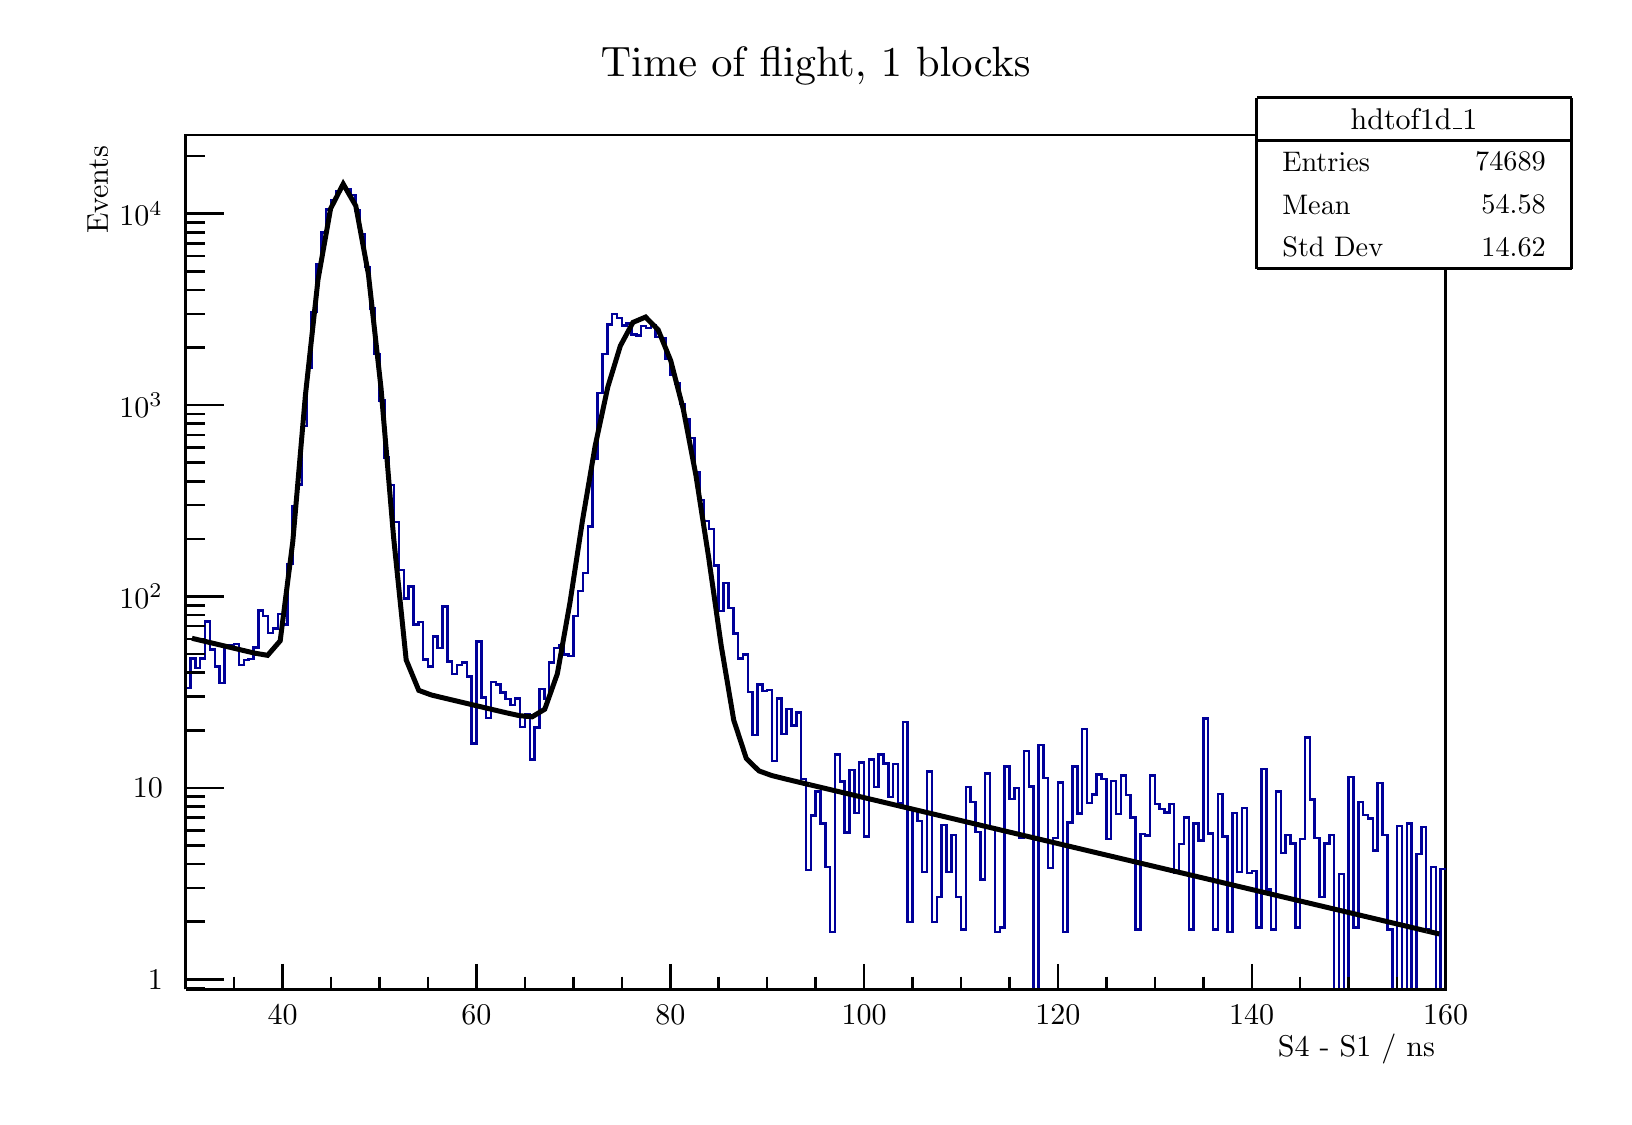
\begin{tikzpicture}
\pgfdeclareplotmark{cross} {
\pgfpathmoveto{\pgfpoint{-0.3\pgfplotmarksize}{\pgfplotmarksize}}
\pgfpathlineto{\pgfpoint{+0.3\pgfplotmarksize}{\pgfplotmarksize}}
\pgfpathlineto{\pgfpoint{+0.3\pgfplotmarksize}{0.3\pgfplotmarksize}}
\pgfpathlineto{\pgfpoint{+1\pgfplotmarksize}{0.3\pgfplotmarksize}}
\pgfpathlineto{\pgfpoint{+1\pgfplotmarksize}{-0.3\pgfplotmarksize}}
\pgfpathlineto{\pgfpoint{+0.3\pgfplotmarksize}{-0.3\pgfplotmarksize}}
\pgfpathlineto{\pgfpoint{+0.3\pgfplotmarksize}{-1.\pgfplotmarksize}}
\pgfpathlineto{\pgfpoint{-0.3\pgfplotmarksize}{-1.\pgfplotmarksize}}
\pgfpathlineto{\pgfpoint{-0.3\pgfplotmarksize}{-0.3\pgfplotmarksize}}
\pgfpathlineto{\pgfpoint{-1.\pgfplotmarksize}{-0.3\pgfplotmarksize}}
\pgfpathlineto{\pgfpoint{-1.\pgfplotmarksize}{0.3\pgfplotmarksize}}
\pgfpathlineto{\pgfpoint{-0.3\pgfplotmarksize}{0.3\pgfplotmarksize}}
\pgfpathclose
\pgfusepathqstroke
}
\pgfdeclareplotmark{cross*} {
\pgfpathmoveto{\pgfpoint{-0.3\pgfplotmarksize}{\pgfplotmarksize}}
\pgfpathlineto{\pgfpoint{+0.3\pgfplotmarksize}{\pgfplotmarksize}}
\pgfpathlineto{\pgfpoint{+0.3\pgfplotmarksize}{0.3\pgfplotmarksize}}
\pgfpathlineto{\pgfpoint{+1\pgfplotmarksize}{0.3\pgfplotmarksize}}
\pgfpathlineto{\pgfpoint{+1\pgfplotmarksize}{-0.3\pgfplotmarksize}}
\pgfpathlineto{\pgfpoint{+0.3\pgfplotmarksize}{-0.3\pgfplotmarksize}}
\pgfpathlineto{\pgfpoint{+0.3\pgfplotmarksize}{-1.\pgfplotmarksize}}
\pgfpathlineto{\pgfpoint{-0.3\pgfplotmarksize}{-1.\pgfplotmarksize}}
\pgfpathlineto{\pgfpoint{-0.3\pgfplotmarksize}{-0.3\pgfplotmarksize}}
\pgfpathlineto{\pgfpoint{-1.\pgfplotmarksize}{-0.3\pgfplotmarksize}}
\pgfpathlineto{\pgfpoint{-1.\pgfplotmarksize}{0.3\pgfplotmarksize}}
\pgfpathlineto{\pgfpoint{-0.3\pgfplotmarksize}{0.3\pgfplotmarksize}}
\pgfpathclose
\pgfusepathqfillstroke
}
\pgfdeclareplotmark{newstar} {
\pgfpathmoveto{\pgfqpoint{0pt}{\pgfplotmarksize}}
\pgfpathlineto{\pgfqpointpolar{44}{0.5\pgfplotmarksize}}
\pgfpathlineto{\pgfqpointpolar{18}{\pgfplotmarksize}}
\pgfpathlineto{\pgfqpointpolar{-20}{0.5\pgfplotmarksize}}
\pgfpathlineto{\pgfqpointpolar{-54}{\pgfplotmarksize}}
\pgfpathlineto{\pgfqpointpolar{-90}{0.5\pgfplotmarksize}}
\pgfpathlineto{\pgfqpointpolar{234}{\pgfplotmarksize}}
\pgfpathlineto{\pgfqpointpolar{198}{0.5\pgfplotmarksize}}
\pgfpathlineto{\pgfqpointpolar{162}{\pgfplotmarksize}}
\pgfpathlineto{\pgfqpointpolar{134}{0.5\pgfplotmarksize}}
\pgfpathclose
\pgfusepathqstroke
}
\pgfdeclareplotmark{newstar*} {
\pgfpathmoveto{\pgfqpoint{0pt}{\pgfplotmarksize}}
\pgfpathlineto{\pgfqpointpolar{44}{0.5\pgfplotmarksize}}
\pgfpathlineto{\pgfqpointpolar{18}{\pgfplotmarksize}}
\pgfpathlineto{\pgfqpointpolar{-20}{0.5\pgfplotmarksize}}
\pgfpathlineto{\pgfqpointpolar{-54}{\pgfplotmarksize}}
\pgfpathlineto{\pgfqpointpolar{-90}{0.5\pgfplotmarksize}}
\pgfpathlineto{\pgfqpointpolar{234}{\pgfplotmarksize}}
\pgfpathlineto{\pgfqpointpolar{198}{0.5\pgfplotmarksize}}
\pgfpathlineto{\pgfqpointpolar{162}{\pgfplotmarksize}}
\pgfpathlineto{\pgfqpointpolar{134}{0.5\pgfplotmarksize}}
\pgfpathclose
\pgfusepathqfillstroke
}
\definecolor{c}{rgb}{1,1,1};
\draw [color=c, fill=c] (0,0) rectangle (20,13.5632);
\draw [color=c, fill=c] (2,1.35632) rectangle (18,12.2069);
\definecolor{c}{rgb}{0,0,0};
\draw [c,line width=0.9] (2,1.35632) -- (2,12.2069) -- (18,12.2069) -- (18,1.35632) -- (2,1.35632);
\definecolor{c}{rgb}{1,1,1};
\draw [color=c, fill=c] (2,1.35632) rectangle (18,12.2069);
\definecolor{c}{rgb}{0,0,0};
\draw [c,line width=0.9] (2,1.35632) -- (2,12.2069) -- (18,12.2069) -- (18,1.35632) -- (2,1.35632);
\definecolor{c}{rgb}{0,0,0.6};
\draw [c,line width=0.9] (2,5.18151) -- (2.06154,5.18151) -- (2.06154,5.55608) -- (2.12308,5.55608) -- (2.12308,5.43961) -- (2.18462,5.43961) -- (2.18462,5.55581) -- (2.24615,5.55581) -- (2.24615,6.03099) -- (2.30769,6.03099) -- (2.30769,5.671) --
 (2.36923,5.671) -- (2.36923,5.45689) -- (2.43077,5.45689) -- (2.43077,5.24567) -- (2.49231,5.24567) -- (2.49231,5.73078) -- (2.55385,5.73078) -- (2.55385,5.72665) -- (2.61538,5.72665) -- (2.61538,5.74226) -- (2.67692,5.74226) -- (2.67692,5.47851) --
 (2.73846,5.47851) -- (2.73846,5.53808) -- (2.8,5.53808) -- (2.8,5.54976) -- (2.86154,5.54976) -- (2.86154,5.69856) -- (2.92308,5.69856) -- (2.92308,6.16999) -- (2.98462,6.16999) -- (2.98462,6.10032) -- (3.04615,6.10032) -- (3.04615,5.88449) --
 (3.10769,5.88449) -- (3.10769,5.93992) -- (3.16923,5.93992) -- (3.16923,6.12156) -- (3.23077,6.12156) -- (3.23077,5.99356) -- (3.29231,5.99356) -- (3.29231,6.75831) -- (3.35385,6.75831) -- (3.35385,7.49725) -- (3.41538,7.49725) -- (3.41538,7.76618)
 -- (3.47692,7.76618) -- (3.47692,8.5123) -- (3.53846,8.5123) -- (3.53846,9.25065) -- (3.6,9.25065) -- (3.6,9.95823) -- (3.66154,9.95823) -- (3.66154,10.5598) -- (3.72308,10.5598) -- (3.72308,10.9657) -- (3.78462,10.9657) -- (3.78462,11.2595) --
 (3.84615,11.2595) -- (3.84615,11.3826) -- (3.90769,11.3826) -- (3.90769,11.4937) -- (3.96923,11.4937) -- (3.96923,11.5322) -- (4.03077,11.5322) -- (4.03077,11.5125) -- (4.09231,11.5125) -- (4.09231,11.4476) -- (4.15385,11.4476) -- (4.15385,11.2503)
 -- (4.21538,11.2503) -- (4.21538,10.9505) -- (4.27692,10.9505) -- (4.27692,10.5305) -- (4.33846,10.5305) -- (4.33846,10.0019) -- (4.4,10.0019) -- (4.4,9.42602) -- (4.46154,9.42602) -- (4.46154,8.83371) -- (4.52308,8.83371) -- (4.52308,8.11005) --
 (4.58462,8.11005) -- (4.58462,7.76378) -- (4.64615,7.76378) -- (4.64615,7.29171) -- (4.70769,7.29171) -- (4.70769,6.67972) -- (4.76923,6.67972) -- (4.76923,6.32169) -- (4.83077,6.32169) -- (4.83077,6.47204) -- (4.89231,6.47204) -- (4.89231,5.993) --
 (4.95385,5.993) -- (4.95385,6.02017) -- (5.01538,6.02017) -- (5.01538,5.54748) -- (5.07692,5.54748) -- (5.07692,5.45714) -- (5.13846,5.45714) -- (5.13846,5.83864) -- (5.2,5.83864) -- (5.2,5.69096) -- (5.26154,5.69096) -- (5.26154,6.21606) --
 (5.32308,6.21606) -- (5.32308,5.51754) -- (5.38462,5.51754) -- (5.38462,5.35984) -- (5.44615,5.35984) -- (5.44615,5.47524) -- (5.50769,5.47524) -- (5.50769,5.50812) -- (5.56923,5.50812) -- (5.56923,5.32886) -- (5.63077,5.32886) -- (5.63077,4.47719)
 -- (5.69231,4.47719) -- (5.69231,5.77627) -- (5.75385,5.77627) -- (5.75385,5.06195) -- (5.81538,5.06195) -- (5.81538,4.80233) -- (5.87692,4.80233) -- (5.87692,5.25956) -- (5.93846,5.25956) -- (5.93846,5.22936) -- (6,5.22936) -- (6,5.12667) --
 (6.06154,5.12667) -- (6.06154,5.04604) -- (6.12308,5.04604) -- (6.12308,4.96718) -- (6.18462,4.96718) -- (6.18462,5.05252) -- (6.24615,5.05252) -- (6.24615,4.68623) -- (6.30769,4.68623) -- (6.30769,4.85157) -- (6.36923,4.85157) -- (6.36923,4.2741)
 -- (6.43077,4.2741) -- (6.43077,4.68523) -- (6.49231,4.68523) -- (6.49231,5.16964) -- (6.55385,5.16964) -- (6.55385,5.0443) -- (6.61538,5.0443) -- (6.61538,5.50863) -- (6.67692,5.50863) -- (6.67692,5.68975) -- (6.73846,5.68975) -- (6.73846,5.72166)
 -- (6.8,5.72166) -- (6.8,5.60763) -- (6.86154,5.60763) -- (6.86154,5.58722) -- (6.92308,5.58722) -- (6.92308,6.09935) -- (6.98462,6.09935) -- (6.98462,6.41753) -- (7.04615,6.41753) -- (7.04615,6.64659) -- (7.10769,6.64659) -- (7.10769,7.2355) --
 (7.16923,7.2355) -- (7.16923,8.09892) -- (7.23077,8.09892) -- (7.23077,8.93136) -- (7.29231,8.93136) -- (7.29231,9.42351) -- (7.35385,9.42351) -- (7.35385,9.79794) -- (7.41538,9.79794) -- (7.41538,9.93183) -- (7.47692,9.93183) -- (7.47692,9.8799) --
 (7.53846,9.8799) -- (7.53846,9.78722) -- (7.6,9.78722) -- (7.6,9.81608) -- (7.66154,9.81608) -- (7.66154,9.67331) -- (7.72308,9.67331) -- (7.72308,9.65902) -- (7.78462,9.65902) -- (7.78462,9.77948) -- (7.84615,9.77948) -- (7.84615,9.75876) --
 (7.90769,9.75876) -- (7.90769,9.79026) -- (7.96923,9.79026) -- (7.96923,9.64053) -- (8.03077,9.64053) -- (8.03077,9.63187) -- (8.09231,9.63187) -- (8.09231,9.36831) -- (8.15385,9.36831) -- (8.15385,9.16368) -- (8.21538,9.16368) -- (8.21538,9.05403)
 -- (8.27692,9.05403) -- (8.27692,8.78876) -- (8.33846,8.78876) -- (8.33846,8.603) -- (8.4,8.603) -- (8.4,8.35968) -- (8.46154,8.35968) -- (8.46154,7.91883) -- (8.52308,7.91883) -- (8.52308,7.56846) -- (8.58462,7.56846) -- (8.58462,7.30407) --
 (8.64615,7.30407) -- (8.64615,7.20532) -- (8.70769,7.20532) -- (8.70769,6.74177) -- (8.76923,6.74177) -- (8.76923,6.16352) -- (8.83077,6.16352) -- (8.83077,6.51821) -- (8.89231,6.51821) -- (8.89231,6.20221) -- (8.95385,6.20221) -- (8.95385,5.87638)
 -- (9.01538,5.87638) -- (9.01538,5.55625) -- (9.07692,5.55625) -- (9.07692,5.61066) -- (9.13846,5.61066) -- (9.13846,5.13328) -- (9.2,5.13328) -- (9.2,4.58783) -- (9.26154,4.58783) -- (9.26154,5.23012) -- (9.32308,5.23012) -- (9.32308,5.146) --
 (9.38461,5.146) -- (9.38461,5.15776) -- (9.44615,5.15776) -- (9.44615,4.25767) -- (9.50769,4.25767) -- (9.50769,5.04774) -- (9.56923,5.04774) -- (9.56923,4.60175) -- (9.63077,4.60175) -- (9.63077,4.92009) -- (9.69231,4.92009) -- (9.69231,4.71042) --
 (9.75385,4.71042) -- (9.75385,4.87061) -- (9.81538,4.87061) -- (9.81538,4.02592) -- (9.87692,4.02592) -- (9.87692,2.87449) -- (9.93846,2.87449) -- (9.93846,3.56693) -- (10,3.56693) -- (10,3.87246) -- (10.0615,3.87246) -- (10.0615,3.4613) --
 (10.1231,3.4613) -- (10.1231,2.90853) -- (10.1846,2.90853) -- (10.1846,2.08809) -- (10.2462,2.08809) -- (10.2462,4.33668) -- (10.3077,4.33668) -- (10.3077,3.99697) -- (10.3692,3.99697) -- (10.3692,3.3477) -- (10.4308,3.3477) -- (10.4308,4.13973) --
 (10.4923,4.13973) -- (10.4923,3.59781) -- (10.5538,3.59781) -- (10.5538,4.23774) -- (10.6154,4.23774) -- (10.6154,3.29987) -- (10.6769,3.29987) -- (10.6769,4.27622) -- (10.7385,4.27622) -- (10.7385,3.92545) -- (10.8,3.92545) -- (10.8,4.34213) --
 (10.8615,4.34213) -- (10.8615,4.22691) -- (10.9231,4.22691) -- (10.9231,3.79686) -- (10.9846,3.79686) -- (10.9846,4.22057) -- (11.0462,4.22057) -- (11.0462,3.71905) -- (11.1077,3.71905) -- (11.1077,4.75094) -- (11.1692,4.75094) -- (11.1692,2.20974)
 -- (11.2308,2.20974) -- (11.2308,3.65017) -- (11.2923,3.65017) -- (11.2923,3.492) -- (11.3538,3.492) -- (11.3538,2.84753) -- (11.4154,2.84753) -- (11.4154,4.12337) -- (11.4769,4.12337) -- (11.4769,2.20974) -- (11.5385,2.20974) -- (11.5385,2.53059)
 -- (11.6,2.53059) -- (11.6,3.44296) -- (11.6615,3.44296) -- (11.6615,2.84753) -- (11.7231,2.84753) -- (11.7231,3.31942) -- (11.7846,3.31942) -- (11.7846,2.53059) -- (11.8462,2.53059) -- (11.8462,2.11846) -- (11.9077,2.11846) -- (11.9077,3.92545) --
 (11.9692,3.92545) -- (11.9692,3.73625) -- (12.0308,3.73625) -- (12.0308,3.35377) -- (12.0923,3.35377) -- (12.0923,2.74928) -- (12.1538,2.74928) -- (12.1538,4.09554) -- (12.2154,4.09554) -- (12.2154,3.41687) -- (12.2769,3.41687) -- (12.2769,2.08809)
 -- (12.3385,2.08809) -- (12.3385,2.14272) -- (12.4,2.14272) -- (12.4,4.18641) -- (12.4615,4.18641) -- (12.4615,3.77723) -- (12.5231,3.77723) -- (12.5231,3.91398) -- (12.5846,3.91398) -- (12.5846,3.27829) -- (12.6462,3.27829) -- (12.6462,4.38363) --
 (12.7077,4.38363) -- (12.7077,3.93124) -- (12.7692,3.93124) -- (12.7692,1.35632) -- (12.8308,1.35632) -- (12.8308,4.45728) -- (12.8923,4.45728) -- (12.8923,4.04146) -- (12.9538,4.04146) -- (12.9538,2.89686) -- (13.0154,2.89686) -- (13.0154,3.27649)
 -- (13.0769,3.27649) -- (13.0769,3.98168) -- (13.1385,3.98168) -- (13.1385,2.08809) -- (13.2,2.08809) -- (13.2,3.47404) -- (13.2615,3.47404) -- (13.2615,4.18641) -- (13.3231,4.18641) -- (13.3231,3.58812) -- (13.3846,3.58812) -- (13.3846,4.66074) --
 (13.4462,4.66074) -- (13.4462,3.72096) -- (13.5077,3.72096) -- (13.5077,3.83058) -- (13.5692,3.83058) -- (13.5692,4.08766) -- (13.6308,4.08766) -- (13.6308,4.03023) -- (13.6923,4.03023) -- (13.6923,3.26645) -- (13.7538,3.26645) -- (13.7538,4.00415)
 -- (13.8154,4.00415) -- (13.8154,3.58678) -- (13.8769,3.58678) -- (13.8769,4.07563) -- (13.9385,4.07563) -- (13.9385,3.82377) -- (14,3.82377) -- (14,3.53914) -- (14.0615,3.53914) -- (14.0615,2.11846) -- (14.1231,2.11846) -- (14.1231,3.33056) --
 (14.1846,3.33056) -- (14.1846,3.3096) -- (14.2462,3.3096) -- (14.2462,4.07579) -- (14.3077,4.07579) -- (14.3077,3.70785) -- (14.3692,3.70785) -- (14.3692,3.64917) -- (14.4308,3.64917) -- (14.4308,3.60516) -- (14.4923,3.60516) -- (14.4923,3.70785) --
 (14.5538,3.70785) -- (14.5538,2.83516) -- (14.6154,2.83516) -- (14.6154,3.20139) -- (14.6769,3.20139) -- (14.6769,3.53914) -- (14.7385,3.53914) -- (14.7385,2.11846) -- (14.8,2.11846) -- (14.8,3.46572) -- (14.8615,3.46572) -- (14.8615,3.24538) --
 (14.9231,3.24538) -- (14.9231,4.79484) -- (14.9846,4.79484) -- (14.9846,3.33729) -- (15.0462,3.33729) -- (15.0462,2.11846) -- (15.1077,2.11846) -- (15.1077,3.83614) -- (15.1692,3.83614) -- (15.1692,3.29647) -- (15.2308,3.29647) -- (15.2308,2.08809)
 -- (15.2923,2.08809) -- (15.2923,3.59713) -- (15.3538,3.59713) -- (15.3538,2.85023) -- (15.4154,2.85023) -- (15.4154,3.66286) -- (15.4769,3.66286) -- (15.4769,2.83516) -- (15.5385,2.83516) -- (15.5385,2.86243) -- (15.6,2.86243) -- (15.6,2.14272) --
 (15.6615,2.14272) -- (15.6615,4.15383) -- (15.7231,4.15383) -- (15.7231,2.62199) -- (15.7846,2.62199) -- (15.7846,2.11846) -- (15.8462,2.11846) -- (15.8462,3.87165) -- (15.9077,3.87165) -- (15.9077,3.08614) -- (15.9692,3.08614) -- (15.9692,3.31751)
 -- (16.0308,3.31751) -- (16.0308,3.21207) -- (16.0923,3.21207) -- (16.0923,2.14272) -- (16.1538,2.14272) -- (16.1538,3.26826) -- (16.2154,3.26826) -- (16.2154,4.55325) -- (16.2769,4.55325) -- (16.2769,3.77087) -- (16.3385,3.77087) --
 (16.3385,3.27829) -- (16.4,3.27829) -- (16.4,2.53059) -- (16.4615,2.53059) -- (16.4615,3.21207) -- (16.5231,3.21207) -- (16.5231,3.31751) -- (16.5846,3.31751) -- (16.5846,1.35632) -- (16.6462,1.35632) -- (16.6462,2.81986) -- (16.7077,2.81986) --
 (16.7077,1.35632) -- (16.7692,1.35632) -- (16.7692,4.05445) -- (16.8308,4.05445) -- (16.8308,2.14272) -- (16.8923,2.14272) -- (16.8923,3.7376) -- (16.9538,3.7376) -- (16.9538,3.57313) -- (17.0154,3.57313) -- (17.0154,3.52486) -- (17.0769,3.52486) --
 (17.0769,3.12021) -- (17.1385,3.12021) -- (17.1385,3.98035) -- (17.2,3.98035) -- (17.2,3.31751) -- (17.2615,3.31751) -- (17.2615,2.11846) -- (17.3231,2.11846) -- (17.3231,1.35632) -- (17.3846,1.35632) -- (17.3846,3.43423) -- (17.4462,3.43423) --
 (17.4462,1.35632) -- (17.5077,1.35632) -- (17.5077,3.4613) -- (17.5692,3.4613) -- (17.5692,1.35632) -- (17.6308,1.35632) -- (17.6308,3.07628) -- (17.6923,3.07628) -- (17.6923,3.41932) -- (17.7538,3.41932) -- (17.7538,2.11846) -- (17.8154,2.11846) --
 (17.8154,2.90853) -- (17.8769,2.90853) -- (17.8769,1.35632) -- (17.9385,1.35632) -- (17.9385,2.88244) -- (18,2.88244);
\definecolor{c}{rgb}{0,0,0};
\draw [c,line width=0.9] (2,1.35632) -- (18,1.35632);
\draw [anchor= east] (18,0.596782) node[scale=1.08496, color=c, rotate=0]{ S4 - S1 / ns};
\draw [c,line width=0.9] (3.23077,1.68184) -- (3.23077,1.35632);
\draw [c,line width=0.9] (3.84615,1.51908) -- (3.84615,1.35632);
\draw [c,line width=0.9] (4.46154,1.51908) -- (4.46154,1.35632);
\draw [c,line width=0.9] (5.07692,1.51908) -- (5.07692,1.35632);
\draw [c,line width=0.9] (5.69231,1.68184) -- (5.69231,1.35632);
\draw [c,line width=0.9] (6.30769,1.51908) -- (6.30769,1.35632);
\draw [c,line width=0.9] (6.92308,1.51908) -- (6.92308,1.35632);
\draw [c,line width=0.9] (7.53846,1.51908) -- (7.53846,1.35632);
\draw [c,line width=0.9] (8.15385,1.68184) -- (8.15385,1.35632);
\draw [c,line width=0.9] (8.76923,1.51908) -- (8.76923,1.35632);
\draw [c,line width=0.9] (9.38461,1.51908) -- (9.38461,1.35632);
\draw [c,line width=0.9] (10,1.51908) -- (10,1.35632);
\draw [c,line width=0.9] (10.6154,1.68184) -- (10.6154,1.35632);
\draw [c,line width=0.9] (11.2308,1.51908) -- (11.2308,1.35632);
\draw [c,line width=0.9] (11.8462,1.51908) -- (11.8462,1.35632);
\draw [c,line width=0.9] (12.4615,1.51908) -- (12.4615,1.35632);
\draw [c,line width=0.9] (13.0769,1.68184) -- (13.0769,1.35632);
\draw [c,line width=0.9] (13.6923,1.51908) -- (13.6923,1.35632);
\draw [c,line width=0.9] (14.3077,1.51908) -- (14.3077,1.35632);
\draw [c,line width=0.9] (14.9231,1.51908) -- (14.9231,1.35632);
\draw [c,line width=0.9] (15.5385,1.68184) -- (15.5385,1.35632);
\draw [c,line width=0.9] (16.1538,1.51908) -- (16.1538,1.35632);
\draw [c,line width=0.9] (16.7692,1.51908) -- (16.7692,1.35632);
\draw [c,line width=0.9] (17.3846,1.51908) -- (17.3846,1.35632);
\draw [c,line width=0.9] (18,1.68184) -- (18,1.35632);
\draw [c,line width=0.9] (3.23077,1.68184) -- (3.23077,1.35632);
\draw [c,line width=0.9] (2.61538,1.51908) -- (2.61538,1.35632);
\draw [c,line width=0.9] (2,1.51908) -- (2,1.35632);
\draw [anchor=base] (3.23077,0.908736) node[scale=1.08496, color=c, rotate=0]{40};
\draw [anchor=base] (5.69231,0.908736) node[scale=1.08496, color=c, rotate=0]{60};
\draw [anchor=base] (8.15385,0.908736) node[scale=1.08496, color=c, rotate=0]{80};
\draw [anchor=base] (10.6154,0.908736) node[scale=1.08496, color=c, rotate=0]{100};
\draw [anchor=base] (13.0769,0.908736) node[scale=1.08496, color=c, rotate=0]{120};
\draw [anchor=base] (15.5385,0.908736) node[scale=1.08496, color=c, rotate=0]{140};
\draw [anchor=base] (18,0.908736) node[scale=1.08496, color=c, rotate=0]{160};
\draw [c,line width=0.9] (2,1.35632) -- (2,12.2069);
\draw [anchor= east] (0.88,12.2069) node[scale=1.08496, color=c, rotate=90]{ Events};
\draw [c,line width=0.9] (2.24,1.37274) -- (2,1.37274);
\draw [c,line width=0.9] (2.48,1.48397) -- (2,1.48397);
\draw [anchor= east] (1.844,1.48397) node[scale=1.08496, color=c, rotate=0]{1};
\draw [c,line width=0.9] (2.24,2.21574) -- (2,2.21574);
\draw [c,line width=0.9] (2.24,2.6438) -- (2,2.6438);
\draw [c,line width=0.9] (2.24,2.94751) -- (2,2.94751);
\draw [c,line width=0.9] (2.24,3.18309) -- (2,3.18309);
\draw [c,line width=0.9] (2.24,3.37557) -- (2,3.37557);
\draw [c,line width=0.9] (2.24,3.53831) -- (2,3.53831);
\draw [c,line width=0.9] (2.24,3.67928) -- (2,3.67928);
\draw [c,line width=0.9] (2.24,3.80363) -- (2,3.80363);
\draw [c,line width=0.9] (2.48,3.91486) -- (2,3.91486);
\draw [anchor= east] (1.844,3.91486) node[scale=1.08496, color=c, rotate=0]{10};
\draw [c,line width=0.9] (2.24,4.64663) -- (2,4.64663);
\draw [c,line width=0.9] (2.24,5.07469) -- (2,5.07469);
\draw [c,line width=0.9] (2.24,5.3784) -- (2,5.3784);
\draw [c,line width=0.9] (2.24,5.61398) -- (2,5.61398);
\draw [c,line width=0.9] (2.24,5.80646) -- (2,5.80646);
\draw [c,line width=0.9] (2.24,5.9692) -- (2,5.9692);
\draw [c,line width=0.9] (2.24,6.11017) -- (2,6.11017);
\draw [c,line width=0.9] (2.24,6.23452) -- (2,6.23452);
\draw [c,line width=0.9] (2.48,6.34575) -- (2,6.34575);
\draw [anchor= east] (1.844,6.34575) node[scale=1.08496, color=c, rotate=0]{$10^{2}$};
\draw [c,line width=0.9] (2.24,7.07752) -- (2,7.07752);
\draw [c,line width=0.9] (2.24,7.50558) -- (2,7.50558);
\draw [c,line width=0.9] (2.24,7.80929) -- (2,7.80929);
\draw [c,line width=0.9] (2.24,8.04487) -- (2,8.04487);
\draw [c,line width=0.9] (2.24,8.23735) -- (2,8.23735);
\draw [c,line width=0.9] (2.24,8.40009) -- (2,8.40009);
\draw [c,line width=0.9] (2.24,8.54106) -- (2,8.54106);
\draw [c,line width=0.9] (2.24,8.66541) -- (2,8.66541);
\draw [c,line width=0.9] (2.48,8.77664) -- (2,8.77664);
\draw [anchor= east] (1.844,8.77664) node[scale=1.08496, color=c, rotate=0]{$10^{3}$};
\draw [c,line width=0.9] (2.24,9.50841) -- (2,9.50841);
\draw [c,line width=0.9] (2.24,9.93647) -- (2,9.93647);
\draw [c,line width=0.9] (2.24,10.2402) -- (2,10.2402);
\draw [c,line width=0.9] (2.24,10.4758) -- (2,10.4758);
\draw [c,line width=0.9] (2.24,10.6682) -- (2,10.6682);
\draw [c,line width=0.9] (2.24,10.831) -- (2,10.831);
\draw [c,line width=0.9] (2.24,10.9719) -- (2,10.9719);
\draw [c,line width=0.9] (2.24,11.0963) -- (2,11.0963);
\draw [c,line width=0.9] (2.48,11.2075) -- (2,11.2075);
\draw [anchor= east] (1.844,11.2075) node[scale=1.08496, color=c, rotate=0]{$10^{4}$};
\draw [c,line width=0.9] (2.24,11.9393) -- (2,11.9393);
\definecolor{c}{rgb}{1,1,1};
\draw [color=c, fill=c] (15.6,10.5115) rectangle (19.6,12.6816);
\definecolor{c}{rgb}{0,0,0};
\draw [c,line width=0.9] (15.6,10.5115) -- (19.6,10.5115);
\draw [c,line width=0.9] (19.6,10.5115) -- (19.6,12.6816);
\draw [c,line width=0.9] (19.6,12.6816) -- (15.6,12.6816);
\draw [c,line width=0.9] (15.6,12.6816) -- (15.6,10.5115);
\draw (17.6,12.4103) node[scale=1.08496, color=c, rotate=0]{hdtof1d\_1};
\draw [c,line width=0.9] (15.6,12.1391) -- (19.6,12.1391);
\draw [anchor= west] (15.8,11.8678) node[scale=1.02114, color=c, rotate=0]{Entries };
\draw [anchor= east] (19.4,11.8678) node[scale=1.02114, color=c, rotate=0]{ 74689};
\draw [anchor= west] (15.8,11.3253) node[scale=1.02114, color=c, rotate=0]{Mean  };
\draw [anchor= east] (19.4,11.3253) node[scale=1.02114, color=c, rotate=0]{  54.58};
\draw [anchor= west] (15.8,10.7828) node[scale=1.02114, color=c, rotate=0]{Std Dev   };
\draw [anchor= east] (19.4,10.7828) node[scale=1.02114, color=c, rotate=0]{  14.62};
\draw [c,line width=1.8] (2.08,5.81522) -- (2.24,5.77729) -- (2.4,5.73936) -- (2.56,5.70143) -- (2.72,5.6635) -- (2.88,5.62584) -- (3.04,5.59883) -- (3.2,5.783) -- (3.36,7.04462) -- (3.52,8.89992) -- (3.68,10.3694) -- (3.84,11.2716) -- (4,11.5852) --
 (4.16,11.3072) -- (4.32,10.4394) -- (4.48,8.9965) -- (4.64,7.0994) -- (4.8,5.54055) -- (4.96,5.1535) -- (5.12,5.09513) -- (5.28,5.05662) -- (5.44,5.01869) -- (5.6,4.98076) -- (5.76,4.94283) -- (5.92,4.90492) -- (6.08,4.86731) -- (6.24,4.83246) --
 (6.4,4.81808) -- (6.56,4.91497) -- (6.72,5.3653) -- (6.88,6.26787) -- (7.04,7.31709) -- (7.2,8.25867) -- (7.36,9.00435) -- (7.52,9.52953) -- (7.68,9.82711) -- (7.84,9.89492) -- (8,9.73249) -- (8.16,9.34039) -- (8.32,8.721) -- (8.48,7.88215) --
 (8.64,6.85117) -- (8.8,5.72561) -- (8.96,4.77556) -- (9.12,4.2879) -- (9.28,4.13137) -- (9.44,4.0733) -- (9.6,4.03279) -- (9.76,3.9946) -- (9.92,3.95665);
\draw [c,line width=1.8] (9.92,3.95665) -- (10.08,3.91871) -- (10.24,3.88078) -- (10.4,3.84285) -- (10.56,3.80492) -- (10.72,3.76699) -- (10.88,3.72906) -- (11.04,3.69113) -- (11.2,3.6532) -- (11.36,3.61527) -- (11.52,3.57734) -- (11.68,3.53941) --
 (11.84,3.50148) -- (12,3.46355) -- (12.16,3.42562) -- (12.32,3.38769) -- (12.48,3.34976) -- (12.64,3.31183) -- (12.8,3.2739) -- (12.96,3.23597) -- (13.12,3.19804) -- (13.28,3.16011) -- (13.44,3.12218) -- (13.6,3.08425) -- (13.76,3.04632) --
 (13.92,3.00839) -- (14.08,2.97046) -- (14.24,2.93253) -- (14.4,2.8946) -- (14.56,2.85667) -- (14.72,2.81874) -- (14.88,2.78081) -- (15.04,2.74288) -- (15.2,2.70495) -- (15.36,2.66702) -- (15.52,2.62909) -- (15.68,2.59116) -- (15.84,2.55323) --
 (16,2.5153) -- (16.16,2.47737) -- (16.32,2.43944) -- (16.48,2.40151) -- (16.64,2.36358) -- (16.8,2.32565) -- (16.96,2.28772) -- (17.12,2.24979) -- (17.28,2.21186) -- (17.44,2.17393) -- (17.6,2.136) -- (17.76,2.09807);
\draw [c,line width=1.8] (17.76,2.09807) -- (17.92,2.06014);
\draw (10,13.0816) node[scale=1.5317, color=c, rotate=0]{Time of flight, 1 blocks};
\end{tikzpicture}

		\end{adjustbox}
		\caption{Example of the time of flight spectrum observed in $S4$ with a combined signal and background function fitted (shown in black)}
		\label{fig:fitEx}
	\end{figure}

	To produce the data used in this analysis, an exponential background function is subtracted. 
	The parameters for this function are taken from the combined signal and background function.

	